% Options for packages loaded elsewhere
\PassOptionsToPackage{unicode}{hyperref}
\PassOptionsToPackage{hyphens}{url}
%
\documentclass[a4paper,oneside,margin=2cm]{book}
\usepackage{listings}

\usepackage{float}
\usepackage{amsmath,amssymb}
\usepackage{iftex}
\usepackage{lmodern}
% Use upquote if available, for straight quotes in verbatim environments
\IfFileExists{upquote.sty}{\usepackage{upquote}}{}
\IfFileExists{microtype.sty}{% use microtype if available
  \usepackage[]{microtype}
  \UseMicrotypeSet[protrusion]{basicmath} % disable protrusion for tt fonts
}{}
\makeatletter
\@ifundefined{KOMAClassName}{% if non-KOMA class
  \IfFileExists{parskip.sty}{%
    \usepackage{parskip}
  }{% else
    \setlength{\parindent}{0pt}
    \setlength{\parskip}{6pt plus 2pt minus 1pt}}
}{% if KOMA class
  \KOMAoptions{parskip=half}}
\makeatother
\usepackage{xcolor}
\usepackage{color}
\usepackage{fancyvrb}
\newcommand{\VerbBar}{|}
\newcommand{\VERB}{\Verb[commandchars=\\\{\}]}
\DefineVerbatimEnvironment{Highlighting}{Verbatim}{commandchars=\\\{\}}
% Add ',fontsize=\small' for more characters per line
\newenvironment{Shaded}{}{}
\newcommand{\AlertTok}[1]{\textcolor[rgb]{1.00,0.00,0.00}{\textbf{#1}}}
\newcommand{\AnnotationTok}[1]{\textcolor[rgb]{0.38,0.63,0.69}{\textbf{\textit{#1}}}}
\newcommand{\AttributeTok}[1]{\textcolor[rgb]{0.49,0.56,0.16}{#1}}
\newcommand{\BaseNTok}[1]{\textcolor[rgb]{0.25,0.63,0.44}{#1}}
\newcommand{\BuiltInTok}[1]{\textcolor[rgb]{0.00,0.50,0.00}{#1}}
\newcommand{\CharTok}[1]{\textcolor[rgb]{0.25,0.44,0.63}{#1}}
\newcommand{\CommentTok}[1]{\textcolor[rgb]{0.38,0.63,0.69}{\textit{#1}}}
\newcommand{\CommentVarTok}[1]{\textcolor[rgb]{0.38,0.63,0.69}{\textbf{\textit{#1}}}}
\newcommand{\ConstantTok}[1]{\textcolor[rgb]{0.53,0.00,0.00}{#1}}
\newcommand{\ControlFlowTok}[1]{\textcolor[rgb]{0.00,0.44,0.13}{\textbf{#1}}}
\newcommand{\DataTypeTok}[1]{\textcolor[rgb]{0.56,0.13,0.00}{#1}}
\newcommand{\DecValTok}[1]{\textcolor[rgb]{0.25,0.63,0.44}{#1}}
\newcommand{\DocumentationTok}[1]{\textcolor[rgb]{0.73,0.13,0.13}{\textit{#1}}}
\newcommand{\ErrorTok}[1]{\textcolor[rgb]{1.00,0.00,0.00}{\textbf{#1}}}
\newcommand{\ExtensionTok}[1]{#1}
\newcommand{\FloatTok}[1]{\textcolor[rgb]{0.25,0.63,0.44}{#1}}
\newcommand{\FunctionTok}[1]{\textcolor[rgb]{0.02,0.16,0.49}{#1}}
\newcommand{\ImportTok}[1]{\textcolor[rgb]{0.00,0.50,0.00}{\textbf{#1}}}
\newcommand{\InformationTok}[1]{\textcolor[rgb]{0.38,0.63,0.69}{\textbf{\textit{#1}}}}
\newcommand{\KeywordTok}[1]{\textcolor[rgb]{0.00,0.44,0.13}{\textbf{#1}}}
\newcommand{\NormalTok}[1]{#1}
\newcommand{\OperatorTok}[1]{\textcolor[rgb]{0.40,0.40,0.40}{#1}}
\newcommand{\OtherTok}[1]{\textcolor[rgb]{0.00,0.44,0.13}{#1}}
\newcommand{\PreprocessorTok}[1]{\textcolor[rgb]{0.74,0.48,0.00}{#1}}
\newcommand{\RegionMarkerTok}[1]{#1}
\newcommand{\SpecialCharTok}[1]{\textcolor[rgb]{0.25,0.44,0.63}{#1}}
\newcommand{\SpecialStringTok}[1]{\textcolor[rgb]{0.73,0.40,0.53}{#1}}
\newcommand{\StringTok}[1]{\textcolor[rgb]{0.25,0.44,0.63}{#1}}
\newcommand{\VariableTok}[1]{\textcolor[rgb]{0.10,0.09,0.49}{#1}}
\newcommand{\VerbatimStringTok}[1]{\textcolor[rgb]{0.25,0.44,0.63}{#1}}
\newcommand{\WarningTok}[1]{\textcolor[rgb]{0.38,0.63,0.69}{\textbf{\textit{#1}}}}
\usepackage{longtable,booktabs,array}
\usepackage{calc} % for calculating minipage widths
% Correct order of tables after \paragraph or \subparagraph
\usepackage{etoolbox}
\makeatletter
\patchcmd\longtable{\par}{\if@noskipsec\mbox{}\fi\par}{}{}
\makeatother
% Allow footnotes in longtable head/foot
\IfFileExists{footnotehyper.sty}{\usepackage{footnotehyper}}{\usepackage{footnote}}
\makesavenoteenv{longtable}
\usepackage{graphicx}
\makeatletter
\def\maxwidth{\ifdim\Gin@nat@width>\linewidth\linewidth\else\Gin@nat@width\fi}
\def\maxheight{\ifdim\Gin@nat@height>\textheight\textheight\else\Gin@nat@height\fi}
\makeatother
% Scale images if necessary, so that they will not overflow the page
% margins by default, and it is still possible to overwrite the defaults
% using explicit options in \includegraphics[width, height, ...]{}
\setkeys{Gin}{width=\maxwidth,height=\maxheight,keepaspectratio}
% Set default figure placement to htbp
\makeatletter
\def\fps@figure{htbp}
\makeatother
\setlength{\emergencystretch}{3em} % prevent overfull lines
\providecommand{\tightlist}{%
  \setlength{\itemsep}{0pt}\setlength{\parskip}{0pt}}
\setcounter{secnumdepth}{-\maxdimen} % remove section numbering
\ifLuaTeX
  \usepackage{selnolig}  % disable illegal ligatures
\fi
\IfFileExists{bookmark.sty}{\usepackage{bookmark}}{\usepackage{hyperref}}
\IfFileExists{xurl.sty}{\usepackage{xurl}}{} % add URL line breaks if available
\urlstyle{same}

\title{IBM TechExchange EMEA 2024 - lab 2078}
\author{Fabio Alessandro ``Fale'' Locati}
\date{v2024-01-23}

\begin{document}
\maketitle
\tableofcontents
\chapter{Ansible}
\hypertarget{check-the-prerequisites}{%
\section{Check the Prerequisites}\label{check-the-prerequisites}}

\hypertarget{objective}{%
\subsection{Objective}\label{objective}}

\begin{itemize}
  \item Understand the lab topology and how to access the environment.
  \item Understand how to work the workshop exercises
  \item Understand challenge labs
\end{itemize}

These first few lab exercises will be exploring the command-line utilities of the Ansible Automation Platform. This includes:

\begin{itemize}
  \item \href{https://github.com/ansible/ansible-navigator}{ansible-navigator} - a command line utility and text-based user interface (TUI) for running and developing Ansible automation content.
  \item \href{https://docs.ansible.com/core.html}{ansible-core} - the base executable that provides the framework, language and functions that underpin the Ansible Automation Platform. It also includes various cli tools like \texttt{ansible}, \texttt{ansible-playbook} and \texttt{ansible-doc}. Ansible Core acts as the bridge between the upstream community with the free and open source Ansible and connects it to the downstream enterprise automation offering from Red Hat, the Ansible Automation Platform.
\item
  \href{https://docs.ansible.com/automation-controller/latest/html/userguide/execution_environments.html}{Execution
  Environments} - not specifically covered in this workshop because the
  built-in Ansible Execution Environments already included all the Red
  Hat supported collections which includes all the collections we use
  for this workshop. Execution Environments are container images that
  can be utilized as Ansible execution.
\item
  \href{https://github.com/ansible/ansible-builder}{ansible-builder} -
  not specifically covered in this workshop, \texttt{ansible-builder} is
  a command line utility to automate the process of building Execution
  Environments.
\end{itemize}

If you need more information on new Ansible Automation Platform
components bookmark this landing page \url{https://red.ht/AAP-20}

\hypertarget{guide}{%
\subsection{Guide}\label{guide}}

\hypertarget{your-lab-environment}{%
\subsubsection{Your Lab Environment}\label{your-lab-environment}}

In this lab you work in a pre-configured lab environment. You will have
access to the following hosts:

\begin{longtable}[]{@{}ll@{}}
\toprule\noalign{}
Role & Inventory name \\
\midrule\noalign{}
\endhead
\bottomrule\noalign{}
\endlastfoot
    Ansible Control Host & 10.3.48.100 \\
    Managed Host & 10.3.48.[100+PARTICIPANT\_ID] \\
\end{longtable}

\hypertarget{step-1---access-the-environment}{%
\subsubsection{Step 1 - Access the
Environment}\label{step-1---access-the-environment}}

You can access the environment, by connecting via SSH to the Ansible Control Host:


\begin{Highlighting}[]
  \NormalTok{ssh USER@10.3.48.100}
\end{Highlighting}

\hypertarget{step-2---using-the-terminal}{%
\subsubsection{Step 2 - Using the
Terminal}\label{step-2---using-the-terminal}}

Create and navigate to the \texttt{rhel-workshop} directory on the Ansible control
node terminal.

\begin{Shaded}
\begin{Highlighting}[]
    \ExtensionTok{[student@controller \textasciitilde{}]}\ExtensionTok{$ mkdir \textasciitilde{}/rhel{-}workshop/}
    \ExtensionTok{[student@controller \textasciitilde{}]}\ExtensionTok{$ cd \textasciitilde{}/rhel{-}workshop/}
    \ExtensionTok{[student@controller rhel{-}workshop]}\ExtensionTok{$}\NormalTok{ pwd}
    \NormalTok{/home/student/rhel{-}workshop}
    \ExtensionTok{[student@controller rhel{-}workshop]}\ExtensionTok{$}
\end{Highlighting}
\end{Shaded}

\begin{itemize}
\tightlist
\item
  \texttt{\textasciitilde{}} - the tilde in this context is a shortcut
  for the home directory, i.e.~\texttt{/home/student}
\item
  \texttt{mkdir} - Linux command to create a directory
\item
  \texttt{cd} - Linux command to change directory
\item
  \texttt{pwd} - Linux command for print working directory. This will
  show the full path to the current working directory.
\end{itemize}

\hypertarget{step-3---examining-execution-environments}{%
\subsubsection{Step 3 - Examining Execution
Environments}\label{step-3---examining-execution-environments}}

Run the \texttt{ansible-navigator} command with the \texttt{images}
argument to look at execution environments configured on the control
node:

\begin{Shaded}
\begin{Highlighting}[]
\ExtensionTok{$}\NormalTok{ ansible{-}navigator images}
\end{Highlighting}
\end{Shaded}

\begin{figure}[H]
\centering
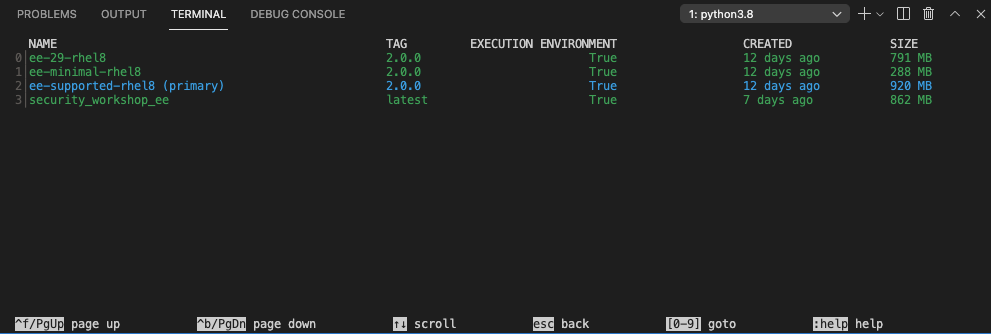
\includegraphics{images/01_navigator-images.png}
\caption{ansible-navigator images}
\end{figure}

\begin{quote}
Note: The output you see might differ from the above output
\end{quote}

This command gives you information about all currently installed
Execution Environments or EEs for short. Investigate an EE by pressing
the corresponding number. For example pressing \textbf{2} with the above
example will open the \texttt{ee-supported-rhel8} execution environment:

\begin{figure}[H]
\centering
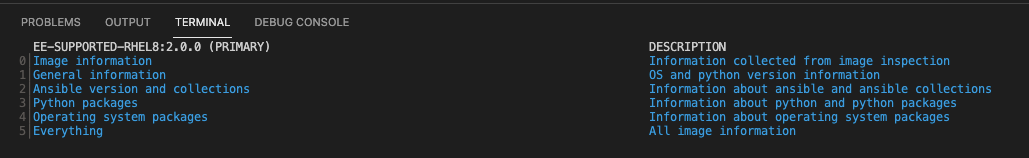
\includegraphics{images/01_navigator-ee-menu.png}
\caption{ee main menu}
\end{figure}

Selecting \texttt{2} for \texttt{Ansible\ version\ and\ collections}
will show us all Ansible Collections installed on that particular EE,
and the version of \texttt{ansible-core}:

\begin{figure}[H]
\centering
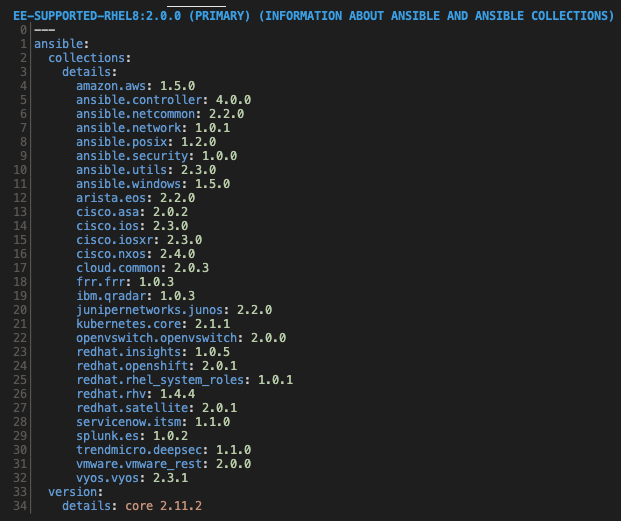
\includegraphics{images/01_navigator-ee-collections.png}
\caption{ee info}
\end{figure}

\hypertarget{step-4---examining-the-ansible-navigator-configuration}{%
\subsubsection{Step 4 - Examining the ansible-navigator
configuration}\label{step-4---examining-the-ansible-navigator-configuration}}

Either use Visual Studio Code to open or use the \texttt{cat} command to
view the contents of the \texttt{ansible-navigator.yml} file. The file
is located in the home directory:

\begin{Shaded}
\begin{Highlighting}[]
\ExtensionTok{$}\NormalTok{ cat \textasciitilde{}/.ansible{-}navigator.yml}
\ExtensionTok{{-}{-}{-}}
\ExtensionTok{ansible{-}navigator:}
  \ExtensionTok{ansible:}
    \ExtensionTok{inventory:}
      \ExtensionTok{entries:}
      \ExtensionTok{{-}}\NormalTok{ \textasciitilde{}/hosts}
  \ExtensionTok{execution{-}environment:}
    \ExtensionTok{image:}\NormalTok{ registry.redhat.io/ansible-automation-platform-24/ee-supported-rhel8:latest}
    \ExtensionTok{enabled:}\NormalTok{ true}
    \ExtensionTok{container{-}engine:}\NormalTok{ podman}
    \ExtensionTok{pull:}
      \ExtensionTok{policy:}\NormalTok{ missing}
    \ExtensionTok{volume{-}mounts:}
    \ExtensionTok{{-}}\NormalTok{ src: }\StringTok{/etc/ansible}
      \ExtensionTok{dest:} \StringTok{/etc/ansible}
\end{Highlighting}
\end{Shaded}

Note the following parameters within the \texttt{.ansible-navigator.yml}
file:

\begin{itemize}
\tightlist
\item
  \texttt{inventories}: shows the location of the ansible inventory
  being used
\item
  \texttt{execution-environment}: where the default execution
  environment is set
\end{itemize}

For a full listing of every configurable knob checkout the
\href{https://ansible.readthedocs.io/projects/navigator/settings/}{documentation}

\hypertarget{step-5---challenge-labs}{%
\subsubsection{Step 5 - Challenge Labs}\label{step-5---challenge-labs}}

You will soon discover that many chapters in this lab guide come with a
``Challenge Lab'' section. These labs are meant to give you a small task
to solve using what you have learned so far. The solution of the task is
shown underneath a warning sign.

\hypertarget{the-ansible-basics}{%
\section{\texorpdfstring{The Ansible Basics
}{The Ansible Basics }}\label{the-ansible-basics}}

\hypertarget{objective}{%
\subsection{Objective}\label{objective}}

In this exercise, we are going to explore the latest Ansible command
line utility \texttt{ansible-navigator} to learn how to work with
inventory files and the listing of modules when needing assistance. The
goal is to familarize yourself with how \texttt{ansible-navigator} works
and how it can be used to enrich your Ansible experience.

This exercise will cover

\begin{itemize}
\tightlist
\item
  Working with inventory files
\item
  Locating and understanding an \texttt{ini} formatted inventory file
\item
  Listing modules and getting help when trying to use them
\end{itemize}

\hypertarget{guide}{%
\subsection{Guide}\label{guide}}

\hypertarget{step-1---work-with-your-inventory}{%
\subsubsection{Step 1 - Work with your
Inventory}\label{step-1---work-with-your-inventory}}

An inventory file is a text file that specifies the nodes that will be
managed by the control machine. The nodes to be managed may include a
list of hostnames or IP addresses of those nodes. The inventory file
allows for nodes to be organized into groups by declaring a host group
name within square brackets ({[}{]}).

To use the \texttt{ansible-navigator} command for host management, you
need to provide an inventory file which defines a list of hosts to be
managed from the control node. In this lab, the inventory is provided by
your instructor. The inventory file is an \texttt{ini} formatted file
listing your hosts, sorted in groups, additionally providing some
variables. It looks like:

\begin{Shaded}
\begin{Highlighting}[]
\ExtensionTok{[web]}
\ExtensionTok{node}\NormalTok{ ansible\_host=}\OperatorTok{\textless{}}\NormalTok{10.3.48.[100+PARTICIPANT_ID]}\OperatorTok{\textgreater{}}

\ExtensionTok{[control]}
\ExtensionTok{controller}\NormalTok{ ansible\_host=10.3.48.100}
\end{Highlighting}
\end{Shaded}

Ansible is already configured to use the inventory specific to your
environment. We will show you in the next step how that is done. For
now, we will execute some simple commands to work with the inventory.

To reference all the inventory hosts, you supply a pattern to the
\texttt{ansible-navigator} command.
\texttt{ansible-navigator\ inventory} has a \texttt{-\/-list} option
which can be useful for displaying all the hosts that are part of an
inventory file including what groups they are associated with.

\begin{Shaded}
\begin{Highlighting}[]
\ExtensionTok{[student@controller}\NormalTok{ rhel\_workshop]$ cd /home/student}
\ExtensionTok{[student@controller}\NormalTok{ \textasciitilde{}]$ ansible{-}navigator inventory }\AttributeTok{{-}{-}list} \AttributeTok{{-}m}\NormalTok{ stdout}
\ExtensionTok{\{}
    \StringTok{"\_meta"}\ExtensionTok{:}\NormalTok{ \{}
        \StringTok{"hostvars"}\ExtensionTok{:}\NormalTok{ \{}
            \StringTok{"controller"}\ExtensionTok{:}\NormalTok{ \{}
                \StringTok{"ansible\_host"}\ExtensionTok{:} \StringTok{"10.3.48.100"}
            \ExtensionTok{\},}
            \StringTok{"node"}\ExtensionTok{:}\NormalTok{ \{}
                \StringTok{"ansible\_host"}\ExtensionTok{:} \StringTok{"10.3.48.101"}
            \ExtensionTok{\}}
        \ExtensionTok{\}}
    \ExtensionTok{\}}\ExtensionTok{,}
    \StringTok{"all"}\ExtensionTok{:}\NormalTok{ \{}
        \StringTok{"children"}\ExtensionTok{:}\NormalTok{ [}
            \StringTok{"control"}\ExtensionTok{,}
            \StringTok{"ungrouped"}\ExtensionTok{,}
            \StringTok{"web"}
        \ExtensionTok{]}
    \ExtensionTok{\}}\ExtensionTok{,}
    \StringTok{"control"}\ExtensionTok{:}\NormalTok{ \{}
        \StringTok{"hosts"}\ExtensionTok{:}\NormalTok{ [}
            \StringTok{"controller"}
        \ExtensionTok{]}
    \ExtensionTok{\}}\ExtensionTok{,}
    \StringTok{"web"}\ExtensionTok{:}\NormalTok{ \{}
        \StringTok{"hosts"}\ExtensionTok{:}\NormalTok{ [}
            \StringTok{"node"}
        \ExtensionTok{]}
    \ExtensionTok{\}}
\ExtensionTok{\}}
\end{Highlighting}
\end{Shaded}

NOTE: \texttt{-m} is short for \texttt{-\/-mode} which allows for the
mode to be switched to standard output instead of using the text-based
user interface (TUI).

If the \texttt{-\/-list} is too verbose, the option of
\texttt{-\/-graph} can be used to provide a more condensed version of
\texttt{-\/-list}.

\begin{Shaded}
\begin{Highlighting}[]
\ExtensionTok{[student@controller}\NormalTok{ \textasciitilde{}]$ ansible{-}navigator inventory }\AttributeTok{{-}{-}graph} \AttributeTok{{-}m}\NormalTok{ stdout}
\ExtensionTok{@all:}
  \KeywordTok{|}\ExtensionTok{{-}{-}@control:}
  \KeywordTok{|}  \KeywordTok{|}\ExtensionTok{{-}{-}controller}
  \KeywordTok{|}\ExtensionTok{{-}{-}@ungrouped:}
  \KeywordTok{|}\ExtensionTok{{-}{-}@web:}
  \KeywordTok{|}  \KeywordTok{|}\ExtensionTok{{-}{-}node}
\end{Highlighting}
\end{Shaded}

We can clearly see that nodes: \texttt{node} is part of the \texttt{web} group, while
\texttt{controller} is part of the \texttt{control} group.

An inventory file can contain a lot more information, it can organize
your hosts in groups or define variables. In our example, the current
inventory has the groups \texttt{web} and \texttt{control}. Run Ansible
with these host patterns and observe the output:

Using the \texttt{ansible-navigator\ inventory} command, we can also run
commands that provide information only for one host or group. For
example, give the following commands a try to see their output.

\begin{Shaded}
\begin{Highlighting}[]
\ExtensionTok{[student@controller}\NormalTok{ \textasciitilde{}]$ ansible{-}navigator inventory }\AttributeTok{{-}{-}graph}\NormalTok{ web }\AttributeTok{{-}m}\NormalTok{ stdout}
\ExtensionTok{[student@controller}\NormalTok{ \textasciitilde{}]$ ansible{-}navigator inventory }\AttributeTok{{-}{-}graph}\NormalTok{ control }\AttributeTok{{-}m}\NormalTok{ stdout}
\ExtensionTok{[student@controller}\NormalTok{ \textasciitilde{}]$ ansible{-}navigator inventory }\AttributeTok{{-}{-}host}\NormalTok{ node }\AttributeTok{{-}m}\NormalTok{ stdout}
\end{Highlighting}
\end{Shaded}

\begin{quote}
\textbf{Tip}

The inventory can contain more data. E.g. if you have hosts that run on
non-standard SSH ports you can put the port number after the hostname
with a colon. Or you could define names specific to Ansible and have
them point to the ``real'' IP or hostname.
\end{quote}

\hypertarget{step-2---listing-modules-and-getting-help}{%
\subsubsection{Step 2 - Listing Modules and Getting
Help}\label{step-2---listing-modules-and-getting-help}}

Ansible Automation Platform comes with multiple supported Execution
Environments (EEs). These EEs come with bundled supported collections
that contain supported content, including modules.

\begin{quote}
\textbf{Tip}

In \texttt{ansible-navigator} exit by pressing the button \texttt{ESC}.
\end{quote}

To browse your available modules first enter interactive mode:

\begin{Shaded}
\begin{Highlighting}[]
\ExtensionTok{$}\NormalTok{ ansible{-}navigator}
\end{Highlighting}
\end{Shaded}

\begin{figure}[H]
\centering
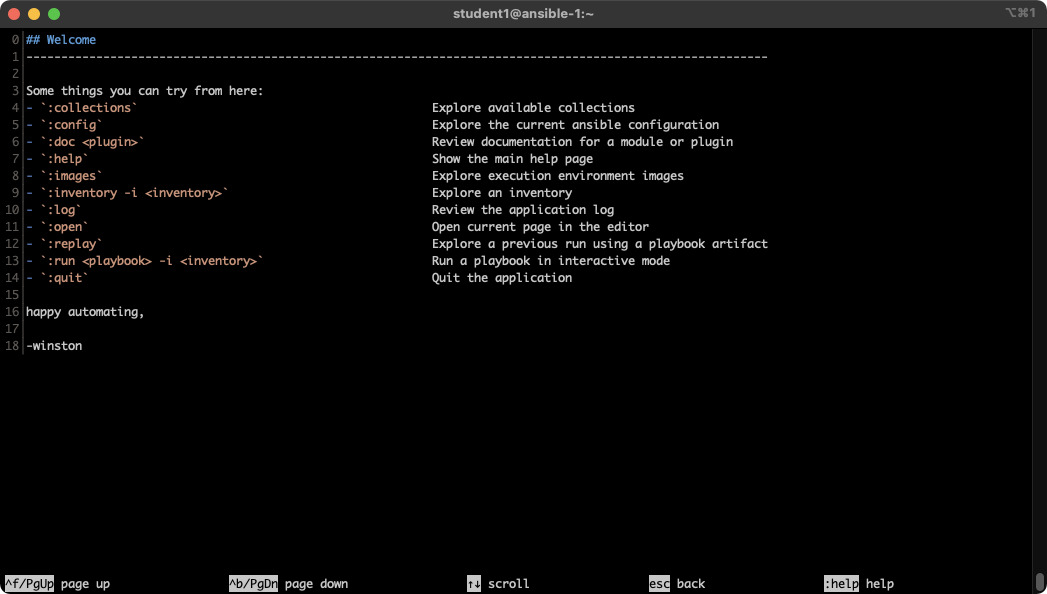
\includegraphics{images/01_interactive-mode.png}
\caption{picture of ansible-navigator}
\end{figure}

First browse a collection by typing \texttt{:collections}

\begin{Shaded}
\begin{Highlighting}[]
\ExtensionTok{:collections}
\end{Highlighting}
\end{Shaded}

\begin{figure}[H]
\centering
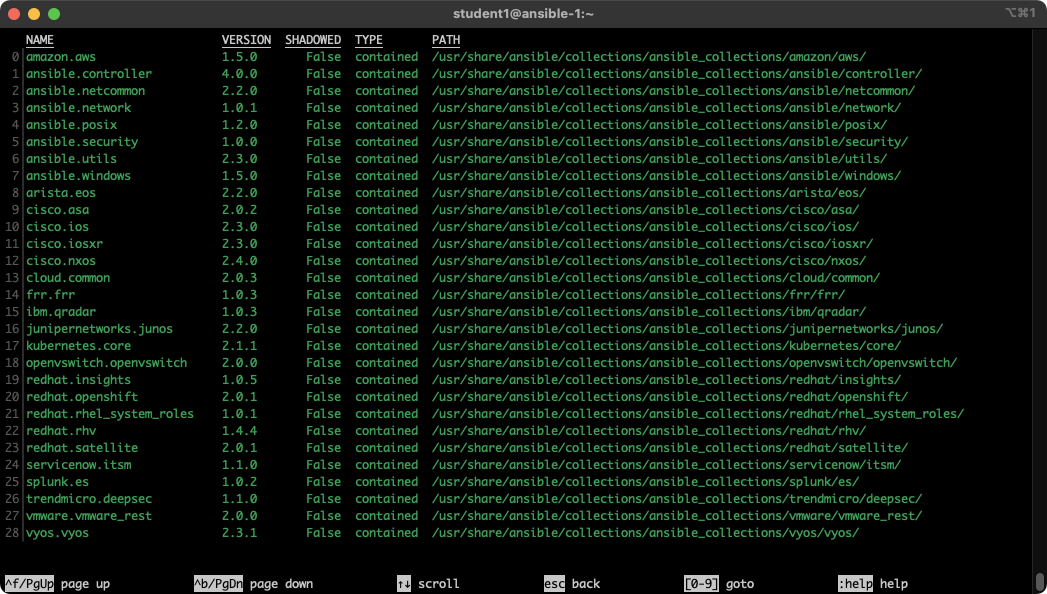
\includegraphics{images/01_interactive-collections.png}
\caption{picture of ansible-navigator}
\end{figure}

To browse the content for a specific collections, type the corresponding
number. For example in the example screenshot above the number
\texttt{0} corresponds to \texttt{amazon.aws} collection. To zoom into
collection type the number \texttt{0}.

\begin{Shaded}
\begin{Highlighting}[]
\ExtensionTok{0}
\end{Highlighting}
\end{Shaded}

\begin{figure}[H]
\centering
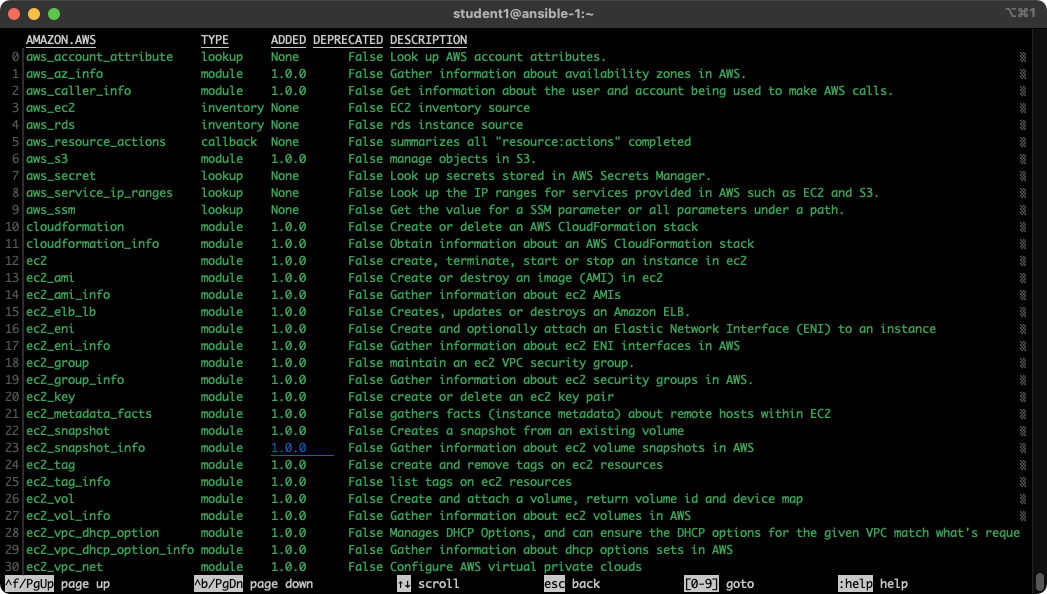
\includegraphics{images/01_interactive-aws.png}
\caption{picture of ansible-navigator}
\end{figure}

Get help for a specific module including usage by zooming in further.
For example the module \texttt{ec2\_metadata\_facts} corresponds to \texttt{3}.

\begin{Shaded}
\begin{Highlighting}[]
\ExtensionTok{:3}
\end{Highlighting}
\end{Shaded}

Scrolling down using the arrow keys or page-up and page-down can show us
documentation and examples.

\begin{figure}[H]
\centering
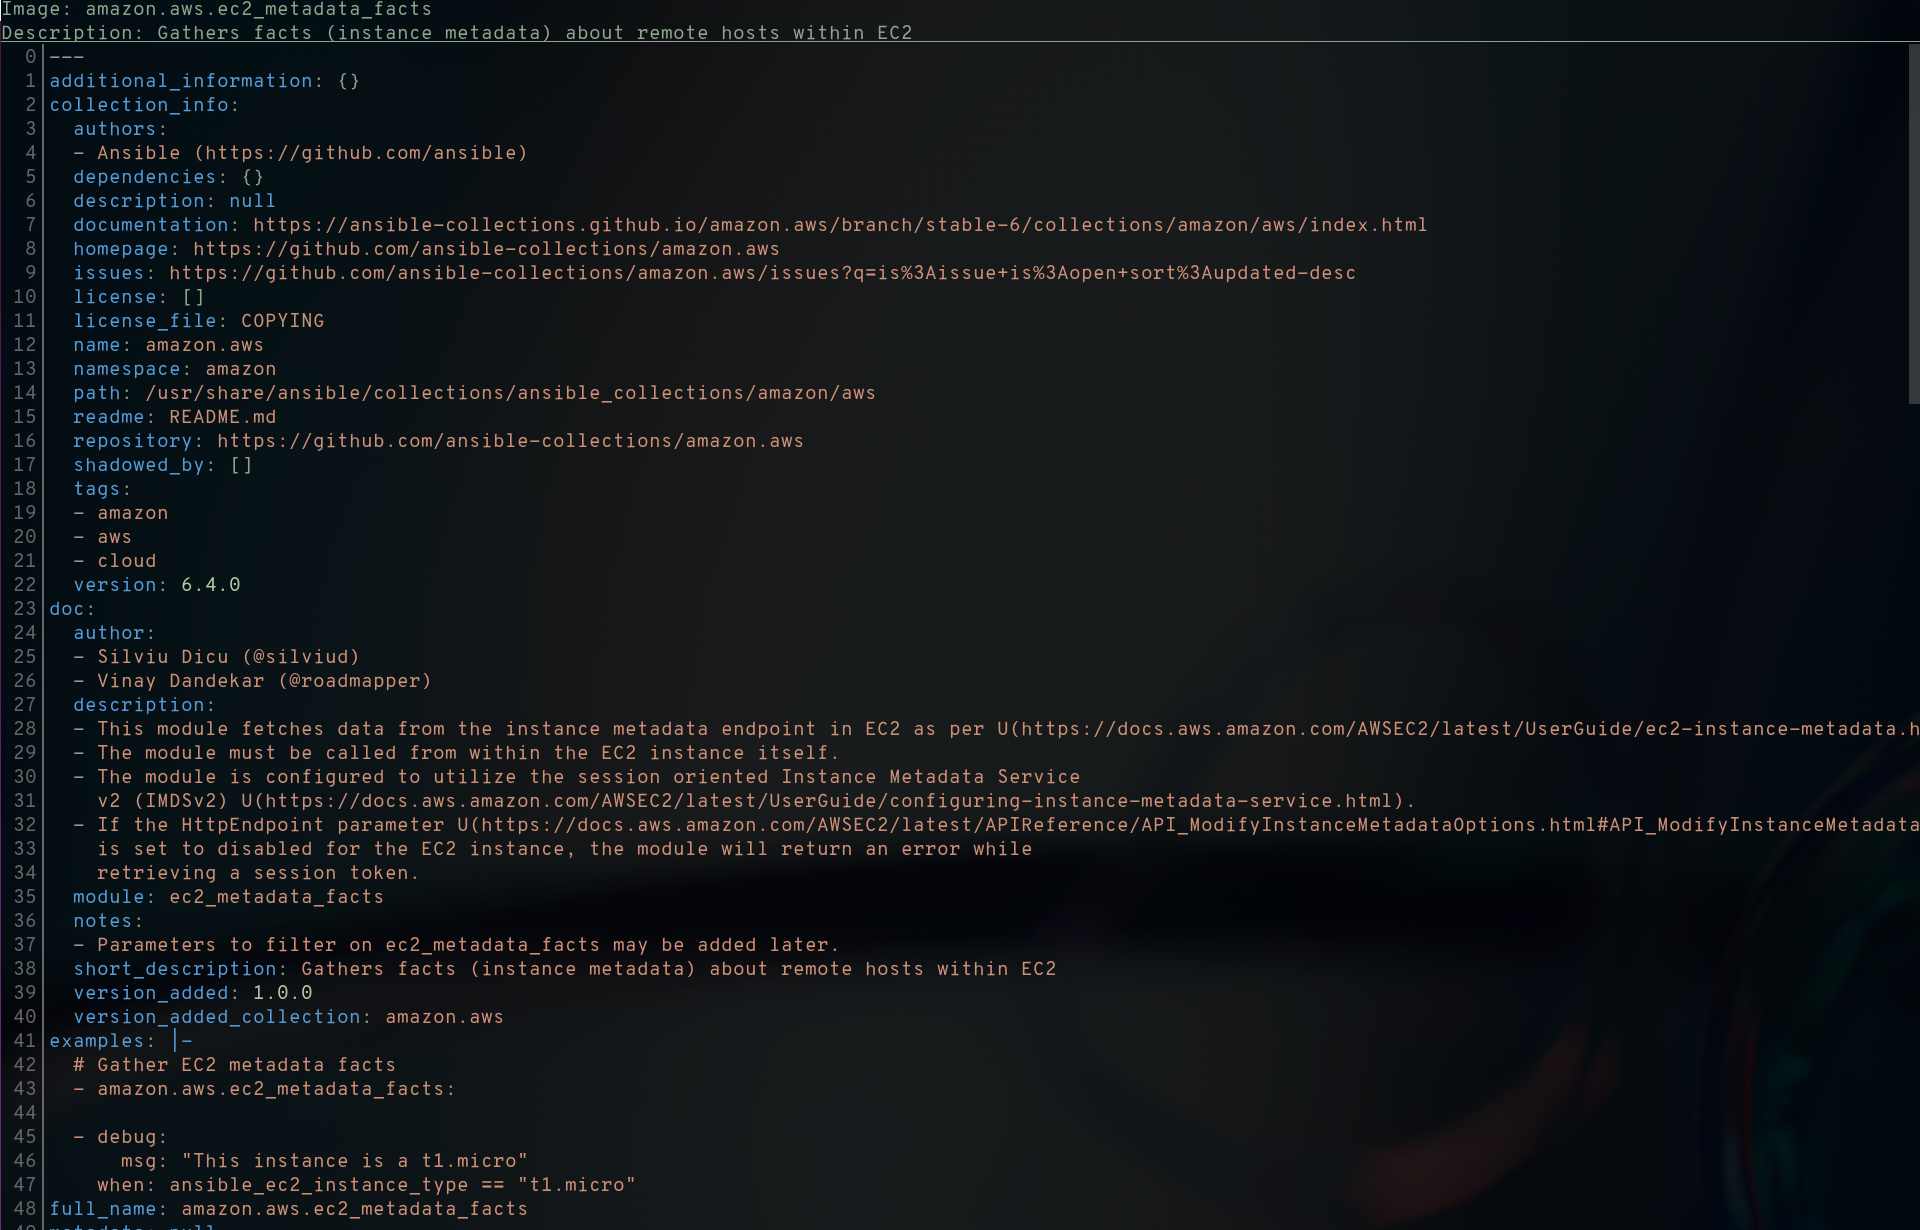
\includegraphics{images/01_interactive-ec2-metadata.png}
\caption{picture of ansible-navigator}
\end{figure}

You can also skip directly to a particular module by simply typing
\texttt{:doc\ namespace.collection.module-name}. For example typing
\texttt{:doc\ amazon.aws.ec2\_metadata\_facts} would skip directly to the final page
shown above.

\begin{quote}
\textbf{Tip}

Different execution environments can have access to different
collections, and different versions of those collections. By using the
built-in documentation you know that it will be accurate for that
particular version of the collection.
\end{quote}

\hypertarget{writing-your-first-playbook}{%
\section{Writing Your First
Playbook}\label{writing-your-first-playbook}}

\hypertarget{objective}{%
\subsection{Objective}\label{objective}}

This exercise covers using Ansible to build an Apache web server on
Red Hat Enterprise Linux. This exercise covers the following Ansible
fundamentals:

\begin{itemize}
\tightlist
\item
  Understanding Ansible module parameters
\item
  Understanding and using the following modules

  \begin{itemize}
  \tightlist
  \item
    \href{https://docs.ansible.com/ansible/latest/modules/dnf_module.html}{dnf
    module}
  \item
    \href{https://docs.ansible.com/ansible/latest/modules/service_module.html}{service
    module}
  \item
    \href{https://docs.ansible.com/ansible/latest/modules/copy_module.html}{copy
    module}
  \end{itemize}
\item
  Understanding
  \href{https://en.wikipedia.org/wiki/Idempotence}{Idempotence} and how
  Ansible modules can be idempotent
\end{itemize}

\hypertarget{guide}{%
\subsection{Guide}\label{guide}}

Playbooks are files which describe the desired configurations or steps
to implement on managed hosts. Playbooks can change lengthy, complex
administrative tasks into easily repeatable routines with predictable
and successful outcomes.

A playbook can have multiple plays and a play can have one or multiple
tasks. In a task a \emph{module} is called, like the modules in the
previous chapter. The goal of a \emph{play} is to map a group of hosts.
The goal of a \emph{task} is to implement modules against those hosts.

\begin{quote}
\textbf{Tip}

Here is a nice analogy: When Ansible modules are the tools in your
workshop, the inventory is the materials and the Playbooks are the
instructions.
\end{quote}

\hypertarget{step-1---playbook-basics}{%
\subsubsection{Step 1 - Playbook
Basics}\label{step-1---playbook-basics}}

Playbooks are text files written in YAML format and therefore need:

\begin{itemize}
\item
  to start with three dashes (\texttt{-\/-\/-})
\item
  proper indentation using spaces and \textbf{not} tabs!
\end{itemize}

There are some important concepts:

\begin{itemize}
\item
  \textbf{hosts}: the managed hosts to perform the tasks on
\item
  \textbf{tasks}: the operations to be performed by invoking Ansible
  modules and passing them the necessary options
\item
  \textbf{become}: privilege escalation in playbooks
\end{itemize}

\begin{quote}
\textbf{Warning}

The ordering of the contents within a Playbook is important, because
Ansible executes plays and tasks in the order they are presented.
\end{quote}

A Playbook should be \textbf{idempotent}, so if a Playbook is run once
to put the hosts in the correct state, it should be safe to run it a
second time and it should make no further changes to the hosts.

\begin{quote}
\textbf{Tip}

Most Ansible modules are idempotent, so it is relatively easy to ensure
this is true.
\end{quote}

\hypertarget{step-2---creating-a-directory-structure-and-file-for-your-playbook}{%
\subsubsection{Step 2 - Creating a Directory Structure and File for your
Playbook}\label{step-2---creating-a-directory-structure-and-file-for-your-playbook}}

Enough theory, it's time to create your first Ansible playbook. In this
lab you create a playbook to set up an Apache web server in three steps:

\begin{enumerate}
\def\labelenumi{\arabic{enumi}.}
\tightlist
\item
  Install httpd package
\item
  Enable/start httpd service
\item
  Copy over an web.html file to each web host
\end{enumerate}

This Playbook makes sure the package containing the Apache web server is
installed on \texttt{node}.

There is a
\href{https://docs.ansible.com/ansible/latest/user_guide/playbooks_best_practices.html}{best
practice} on the preferred directory structures for playbooks. We
strongly encourage you to read and understand these practices as you
develop your Ansible ninja skills. That said, our playbook today is very
basic and creating a complex structure will just confuse things.

Instead, we are going to create a very simple directory structure for
our playbook, and add just a couple of files to it.

On your control host \textbf{ansible}, create a directory called
\texttt{ansible-files} in your home directory and change directories
into it:

\begin{Shaded}
\begin{Highlighting}[]
\ExtensionTok{[student@controller}\NormalTok{ \textasciitilde{}]$ mkdir ansible{-}files}
\ExtensionTok{[student@controller}\NormalTok{ \textasciitilde{}]$ cd ansible{-}files/}
\end{Highlighting}
\end{Shaded}

Add a file called \texttt{apache.yml} with the following content. As
discussed in the previous exercises, use \texttt{vi}/\texttt{vim} or \texttt{nano}.

\begin{Shaded}
\begin{Highlighting}[]
\PreprocessorTok{{-}{-}{-}}
\KeywordTok{{-}}\AttributeTok{ }\FunctionTok{name}\KeywordTok{:}\AttributeTok{ Apache server installed}
\AttributeTok{  }\FunctionTok{hosts}\KeywordTok{:}\AttributeTok{ node}
\AttributeTok{  }\FunctionTok{become}\KeywordTok{:}\AttributeTok{ }\CharTok{True}
\end{Highlighting}
\end{Shaded}

This shows one of Ansible's strengths: The Playbook syntax is easy to
read and understand. In this Playbook:

\begin{itemize}
\tightlist
\item
  A name is given for the play via \texttt{name:}.
\item
  The host to run the playbook against is defined via \texttt{hosts:}.
\item
  We enable user privilege escalation with \texttt{become:}.
\end{itemize}

\begin{quote}
\textbf{Tip}

You obviously need to use privilege escalation to install a package or
run any other task that requires root permissions. This is done in the
Playbook by \texttt{become:\ yes}.
\end{quote}

Now that we've defined the play, let's add a task to get something done.
We will add a task in which dnf will ensure that the Apache package is
installed in the latest version. Modify the file so that it looks like
the following listing:

\begin{Shaded}
\begin{Highlighting}[]
\PreprocessorTok{{-}{-}{-}}
\KeywordTok{{-}}\AttributeTok{ }\FunctionTok{name}\KeywordTok{:}\AttributeTok{ Apache server installed}
\AttributeTok{  }\FunctionTok{hosts}\KeywordTok{:}\AttributeTok{ node}
\AttributeTok{  }\FunctionTok{become}\KeywordTok{:}\AttributeTok{ }\CharTok{True}
\AttributeTok{  }\FunctionTok{tasks}\KeywordTok{:}
\AttributeTok{    }\KeywordTok{{-}}\AttributeTok{ }\FunctionTok{name}\KeywordTok{:}\AttributeTok{ Install Apache}
\AttributeTok{      }\FunctionTok{ansible.builtin.dnf}\KeywordTok{:}
\AttributeTok{        }\FunctionTok{name}\KeywordTok{:}\AttributeTok{ httpd}
\end{Highlighting}
\end{Shaded}

\begin{quote}
\textbf{Tip}

Since playbooks are written in YAML, alignment of the lines and keywords
is crucial. Make sure to vertically align the \emph{t} in \texttt{task}
with the \emph{b} in \texttt{become}. Once you are more familiar with
Ansible, make sure to take some time and study a bit the
\href{https://docs.ansible.com/ansible/latest/reference_appendices/YAMLSyntax.html}{YAML
Syntax}.
\end{quote}

In the added lines:

\begin{itemize}
\tightlist
\item
  We started the tasks part with the keyword \texttt{tasks:}.
\item
  A task is named and the module for the task is referenced. Here it
  uses the \texttt{dnf} module.
\item
  Parameters for the module are added:

  \begin{itemize}
  \tightlist
  \item
    \texttt{name:} to identify the package name
  \item
    \texttt{state:} to define the wanted state of the package
  \end{itemize}
\end{itemize}

\begin{quote}
\textbf{Tip}

The module parameters are individual to each module. If in doubt, look
them up again with \texttt{ansible-doc}.
\end{quote}

Save your playbook and exit your editor.

\hypertarget{step-3---running-the-playbook}{%
\subsubsection{Step 3 - Running the
Playbook}\label{step-3---running-the-playbook}}

With the introduction of Ansible Automation Platform 2, several new key
components are being introduced as a part of the overall developer
experience. Execution environments have been introduced to provide
predictable environments to be used during automation runtime. All
collection dependencies are contained within the execution environment
to ensure that automation created in development environments runs the
same as in production environments.

What do you find within an execution environment?

\begin{itemize}
\tightlist
\item
  RHEL UBI 8
\item
  Ansible 2.9 or Ansible Core 2.11
\item
  Python 3.8
\item
  Any content Collections
\item
  Collection python or binary dependencies.
\end{itemize}

Why use execution environments?

They provide a standardized way to define, build and distribute the
environments that the automation runs in. In a nutshell, Automation
execution environments are container images that allow for easier
administration of Ansible by the platform administrator.

Considering the shift towards containerized execution of automation,
automation development workflow and tooling that existed before Ansible
Automation Platform 2 have had to be reimagined. In short,
\texttt{ansible-navigator} replaces \texttt{ansible-playbook} and other
\texttt{ansible-*} command line utilities.

With this change, Ansible playbooks are executed using the
\texttt{ansible-navigator} command on the control node.

The prerequisites and best practices for using
\texttt{ansible-navigator} have been done for you within this lab.

These include:
\begin{itemize}
\tightlist
\item Installing the \texttt{ansible-navigator} package
\item Creating a default settings \texttt{\textasciitilde{}/.ansible-navigator.yml} for all your projects (optional)
\item All execution environment (EE) logs are stored within the execution folder
\end{itemize}

For more information on the
\href{https://github.com/ansible/ansible-navigator/blob/main/docs/settings.rst}{Ansible
navigator settings}

\begin{quote}
\textbf{Tip}

The parameters for ansible-navigator maybe modified for your specific
environment. The current settings use a default
\texttt{ansible-navigator.yml} for all projects, but a specific
\texttt{ansible-navigator.yml} can be created for each project and is
the recommended practice.
\end{quote}

To run your playbook, use the
\texttt{ansible-navigator\ run\ \textless{}playbook\textgreater{}}
command as follows:

\begin{Shaded}
\begin{Highlighting}[]
\ExtensionTok{[student@controller}\NormalTok{ ansible{-}files]$ ansible{-}navigator run apache.yml}
\end{Highlighting}
\end{Shaded}

\begin{quote}
\textbf{Tip}

The existing \texttt{ansible-navigator.yml} file provides the location
of your inventory file. If this was not set within your
\texttt{ansible-navigator.yml} file, the command to run the playbook
would be:
\texttt{ansible-navigator\ run\ apache.yml\ -i\ \textasciitilde{}/hosts}
\end{quote}

When running the playbook, you'll be displayed a text user interface
(TUI) that displays the play name among other information about the
playbook that is currently run.

\begin{Shaded}
\begin{Highlighting}[]
  \ExtensionTok{PLAY}\NormalTok{ NAME                        OK  CHANGED    UNREACHABLE      FAILED    SKIPPED    IGNORED    IN PROGRESS     TASK COUNT          PROGRESS}
\ExtensionTok{0│Apache}\NormalTok{ server installed           2        1              0           0          0          0              0              2          COMPLETE}
\end{Highlighting}
\end{Shaded}

If you notice, prior to the play name
\texttt{Apache\ server\ installed}, you'll see a \texttt{0}. By pressing
the \texttt{0} key on your keyboard, you will be provided a new window
view displaying the different tasks that ran for the playbook
completion. In this example, those tasks included the ``Gathering
Facts'' and ``Install Apache''. The ``Gathering Facts'' is a built-in
task that runs automatically at the beginning of each play. It collects
information about the managed nodes. Exercises later on will cover this
in more detail. The ``Install Apache'' was the task created within the
\texttt{apache.yml} file that installed \texttt{httpd}.

The display should look something like this:

\begin{Shaded}
\begin{Highlighting}[]
  \ExtensionTok{RESULT}\NormalTok{      HOST  NUMBER      CHANGED       TASK                                                   TASK ACTION           DURATION}
\ExtensionTok{0│OK}\NormalTok{          node          0        False       Gathering Facts                                        gather\_facts                1s}
\ExtensionTok{1│OK}\NormalTok{          node          1         True       Install Apache                        dnf                         4s}
\end{Highlighting}
\end{Shaded}

Taking a closer look, you'll notice that each task is associated with a
number. Task 1, ``Install Apache'', had a change and used the
\texttt{dnf} module. In this case, the change is the installation of
Apache (\texttt{httpd} package) on the host \texttt{node}.

By pressing \texttt{0} or \texttt{1} on your keyboard, you can see
further details of the task being run. If a more traditional output view
is desired, type \texttt{:st} within the text user interface.

Once you've completed, reviewing your Ansible playbook, you can exit out
of the TUI via the Esc key on your keyboard.

\begin{quote}
\textbf{Tip}

The Esc key only takes you back to the previous screen. Once at the main
overview screen an additional Esc key will take you back to the terminal
window.
\end{quote}

Once the playbook has completed, connect to \texttt{node} via SSH to
make sure Apache has been installed:

\begin{Shaded}
\begin{Highlighting}[]
\ExtensionTok{[student@controller}\NormalTok{ ansible{-}files]$ ssh root@10.3.48.[100+PARTICIPANT\_ID]}
\ExtensionTok{Last}\NormalTok{ login: Thu Jan 11 10:35:34 2024 from 10.3.48.100}
\end{Highlighting}
\end{Shaded}

Use the command \texttt{rpm\ -qi\ httpd} to verify httpd is installed:

\begin{Shaded}
\begin{Highlighting}[]
\ExtensionTok{[ec2{-}user@node}\NormalTok{ \textasciitilde{}]$ rpm }\AttributeTok{{-}qi}\NormalTok{ httpd}
\ExtensionTok{Name}\NormalTok{        : httpd}
\ExtensionTok{Version}\NormalTok{     : 2.4.37}
\ExtensionTok{[...]}
\end{Highlighting}
\end{Shaded}

Log out of \texttt{node} with the command \texttt{exit} so that you are
back on the control host and verify the installed package with an
Ansible playbook labeled \texttt{package.yml}

\begin{Shaded}
\begin{Highlighting}[]
\PreprocessorTok{{-}{-}{-}}
\KeywordTok{{-}}\AttributeTok{ }\FunctionTok{name}\KeywordTok{:}\AttributeTok{ Check packages}
\AttributeTok{  }\FunctionTok{hosts}\KeywordTok{:}\AttributeTok{ node}
\AttributeTok{  }\FunctionTok{become}\KeywordTok{:}\AttributeTok{ }\CharTok{True}
\AttributeTok{  }\FunctionTok{vars}\KeywordTok{:}
\AttributeTok{    }\FunctionTok{p}\KeywordTok{:}\AttributeTok{ httpd}
\AttributeTok{  }\FunctionTok{tasks}\KeywordTok{:}
\AttributeTok{    }\KeywordTok{{-}}\AttributeTok{ }\FunctionTok{name}\KeywordTok{:}\AttributeTok{ Gather the packages facts}
\AttributeTok{      }\FunctionTok{ansible.builtin.package\_facts}\KeywordTok{:}
\AttributeTok{        }\FunctionTok{manager}\KeywordTok{:}\AttributeTok{ auto}
\AttributeTok{    }\KeywordTok{{-}}\AttributeTok{ }\FunctionTok{name}\KeywordTok{:}\StringTok{ "Check whether \{\{ p \}\} is installed"}
\AttributeTok{      }\FunctionTok{ansible.builtin.debug}\KeywordTok{:}
\AttributeTok{        }\FunctionTok{msg}\KeywordTok{:}\AttributeTok{ }\StringTok{"\{\{ p \}\} \{\{ ansible\_facts.packages[p][0].version \}\} is installed!"}
\AttributeTok{      }\FunctionTok{when}\KeywordTok{:}\AttributeTok{ p in ansible\_facts.packages}
\end{Highlighting}
\end{Shaded}

You can now run it similarly to the previous one:

\begin{Shaded}
\begin{Highlighting}[]
\ExtensionTok{[student@controller}\NormalTok{ \textasciitilde{}]$ ansible{-}navigator run package.yml }\AttributeTok{{-}m}\NormalTok{ stdout}
\end{Highlighting}
\end{Shaded}

\begin{Shaded}
\begin{Highlighting}[]

\ExtensionTok{PLAY}\NormalTok{ [Check packages] }\PreprocessorTok{**********************************************************}

\ExtensionTok{TASK}\NormalTok{ [Gathering Facts] }\PreprocessorTok{*********************************************************}
\ExtensionTok{ok:} \PreprocessorTok{[}\SpecialStringTok{ansible}\PreprocessorTok{]}

\ExtensionTok{TASK}\NormalTok{ [Gather the packages facts] }\PreprocessorTok{************************************************}
\ExtensionTok{ok:} \PreprocessorTok{[}\SpecialStringTok{ansible}\PreprocessorTok{]}

\ExtensionTok{TASK}\NormalTok{ [Check whether httpd is installed] }\PreprocessorTok{*************************************}
\ExtensionTok{ok:} \PreprocessorTok{[}\SpecialStringTok{ansible}\PreprocessorTok{]}\NormalTok{ =}\OperatorTok{\textgreater{}}\NormalTok{ \{}
    \StringTok{"msg"}\ExtensionTok{:} \StringTok{"httpd 2.4.37 is installed!"}
\NormalTok{\}}

\ExtensionTok{PLAY}\NormalTok{ RECAP }\PreprocessorTok{*********************************************************************}
\ExtensionTok{ansible}\NormalTok{: ok=3  changed=0  unreachable=0  failed=0  skipped=0  rescued=0  ignored=0}
\end{Highlighting}
\end{Shaded}

Run the the \texttt{ansible-navigator\ run\ apache.yml} playbook for a
second time, and compare the output. The output ``CHANGED'' now shows
\texttt{0} instead of \texttt{1} and the color changed from yellow to
green. This makes it easier to spot when changes have occured when
running the Ansible playbook.

\hypertarget{step-4---extend-your-playbook-start-enable-apache}{%
\subsubsection{Step 4 - Extend your Playbook: Start \& Enable
Apache}\label{step-4---extend-your-playbook-start-enable-apache}}

The next part of the Ansible playbook makes sure the Apache application
is enabled and started on \texttt{node}.

On the control host, as your student user, edit the file
\texttt{\textasciitilde{}/ansible-files/apache.yml} to add a second task
using the \texttt{service} module. The Playbook should now look like
this:

\begin{Shaded}
\begin{Highlighting}[]
\PreprocessorTok{{-}{-}{-}}
\KeywordTok{{-}}\AttributeTok{ }\FunctionTok{name}\KeywordTok{:}\AttributeTok{ Apache server installed}
\AttributeTok{  }\FunctionTok{hosts}\KeywordTok{:}\AttributeTok{ node}
\AttributeTok{  }\FunctionTok{become}\KeywordTok{:}\AttributeTok{ }\CharTok{True}
\AttributeTok{  }\FunctionTok{tasks}\KeywordTok{:}
\AttributeTok{    }\KeywordTok{{-}}\AttributeTok{ }\FunctionTok{name}\KeywordTok{:}\AttributeTok{ Install Apache}
\AttributeTok{      }\FunctionTok{ansible.builtin.dnf}\KeywordTok{:}
\AttributeTok{        }\FunctionTok{name}\KeywordTok{:}\AttributeTok{ httpd}
\AttributeTok{    }\KeywordTok{{-}}\AttributeTok{ }\FunctionTok{name}\KeywordTok{:}\AttributeTok{ Apache enabled and running}
\AttributeTok{      }\FunctionTok{ansible.builtin.service}\KeywordTok{:}
\AttributeTok{        }\FunctionTok{name}\KeywordTok{:}\AttributeTok{ httpd}
\AttributeTok{        }\FunctionTok{enabled}\KeywordTok{:}\AttributeTok{ }\CharTok{True}
\AttributeTok{        }\FunctionTok{state}\KeywordTok{:}\AttributeTok{ started}
\end{Highlighting}
\end{Shaded}

What exactly did we do?

\begin{itemize}
\tightlist
\item
  a second task named ``Apache enabled and running'' is created
\item
  a module is specified (\texttt{service})
\item
  The module \texttt{service} takes the name of the service
  (\texttt{httpd}), if it should be permanently set (\texttt{enabled}),
  and its current state (\texttt{started})
\end{itemize}

Thus with the second task we make sure the Apache server is indeed
running on the target machine. Run your extended Playbook:

\begin{Shaded}
\begin{Highlighting}[]
\ExtensionTok{[student@controller}\NormalTok{ \textasciitilde{}]$ ansible{-}navigator run apache.yml}
\end{Highlighting}
\end{Shaded}

Notice in the output, we see the play had \texttt{1} ``CHANGED'' shown
in yellow and if we press \texttt{0} to enter the play output, you can
see that task 2, ``Apache enabled and running'', was the task that
incorporated the latest change by the ``CHANGED'' value being set to
True and highlighted in yellow.

\begin{itemize}
\item
  Run the playbook a second time using \texttt{ansible-navigator} to get
  used to the change in the output.
\item
  Use an Ansible playbook labeled \texttt{service\_state.yml} to make sure the
  Apache (httpd) service is running on \texttt{node}, e.g.~with:
  \texttt{systemctl\ status\ httpd}.
\end{itemize}

\begin{Shaded}
\begin{Highlighting}[]
\PreprocessorTok{{-}{-}{-}}
\KeywordTok{{-}}\AttributeTok{ }\FunctionTok{name}\KeywordTok{:}\AttributeTok{ Check Status}
\AttributeTok{  }\FunctionTok{hosts}\KeywordTok{:}\AttributeTok{ node}
\AttributeTok{  }\FunctionTok{become}\KeywordTok{:}\AttributeTok{ }\CharTok{True}
\AttributeTok{  }\FunctionTok{vars}\KeywordTok{:}
\AttributeTok{    }\FunctionTok{package}\KeywordTok{:}\AttributeTok{ httpd}
\AttributeTok{  }\FunctionTok{tasks}\KeywordTok{:}
\AttributeTok{    }\KeywordTok{{-}}\AttributeTok{ }\FunctionTok{name}\KeywordTok{:}\StringTok{ "Check status of \{\{ package \}\} service"}
\AttributeTok{      }\FunctionTok{ansible.builtin.service\_facts}\KeywordTok{:}
\AttributeTok{      }\FunctionTok{register}\KeywordTok{:}\AttributeTok{ service\_state}
\AttributeTok{    }\KeywordTok{{-}}\AttributeTok{ }\FunctionTok{ansible.builtin.debug}\KeywordTok{:}
\AttributeTok{        }\FunctionTok{var}\KeywordTok{:}\AttributeTok{ service\_state.ansible\_facts.services["\{\{ package \}\}.service"].state}
\end{Highlighting}
\end{Shaded}

\begin{Shaded}
\begin{Highlighting}[]
\ExtensionTok{[student@controller}\NormalTok{ \textasciitilde{}]$ ansible{-}navigator run service\_state.yml}
\end{Highlighting}
\end{Shaded}

\hypertarget{step-5---extend-your-playbook-create-an-web.html}{%
\subsubsection{Step 5 - Extend your Playbook: Create an
web.html}\label{step-5---extend-your-playbook-create-an-web.html}}

Check that the tasks were executed correctly and Apache is accepting
connections: Make an HTTP request using Ansible's \texttt{uri} module in
a playbook named \texttt{check\_httpd.yml} from the control node to
\texttt{node}.

\begin{Shaded}
\begin{Highlighting}[]
\PreprocessorTok{{-}{-}{-}}
\KeywordTok{{-}}\AttributeTok{ }\FunctionTok{name}\KeywordTok{:}\AttributeTok{ Check URL}
\AttributeTok{  }\FunctionTok{hosts}\KeywordTok{:}\AttributeTok{ control}
\AttributeTok{  }\FunctionTok{vars}\KeywordTok{:}
\AttributeTok{    }\FunctionTok{node}\KeywordTok{:}\AttributeTok{ }\StringTok{"[YOUR NODE IP ADDRESS]"}
\AttributeTok{  }\FunctionTok{tasks}\KeywordTok{:}
\AttributeTok{    }\KeywordTok{{-}}\AttributeTok{ }\FunctionTok{name}\KeywordTok{:}\AttributeTok{ Check that you can connect (GET) to a page and it returns a status 200}
\AttributeTok{      }\FunctionTok{ansible.builtin.uri}\KeywordTok{:}
\AttributeTok{        }\FunctionTok{url}\KeywordTok{:}\AttributeTok{ }\StringTok{"http://\{\{ node \}\}"}
\end{Highlighting}
\end{Shaded}

\begin{quote}
\textbf{Warning: Expect a lot of red lines!}
\end{quote}

\begin{Shaded}
\begin{Highlighting}[]
\ExtensionTok{[student@controller}\NormalTok{ \textasciitilde{}]$ ansible{-}navigator run check\_httpd.yml }\AttributeTok{{-}m}\NormalTok{ stdout}
\end{Highlighting}
\end{Shaded}

There are a lot of red lines and an error: As long as there is not at
least an \texttt{web.html} file to be served by Apache, it will throw an
ugly ``HTTP Error 403: Forbidden'' status and Ansible will report an
error.
Also, you are not even seeing the 403 error, since the \texttt{node} port 80 is not reachable due to firewalld's configuration which does not allow connections to be allowed.

Let's start fixing this last issue. To do so, we'll alter the \texttt{apache.yml} file in the following way:

\begin{Shaded}
\begin{Highlighting}[]
\PreprocessorTok{{-}{-}{-}}
\KeywordTok{{-}}\AttributeTok{ }\FunctionTok{name}\KeywordTok{:}\AttributeTok{ Apache server installed}
\AttributeTok{  }\FunctionTok{hosts}\KeywordTok{:}\AttributeTok{ node}
\AttributeTok{  }\FunctionTok{become}\KeywordTok{:}\AttributeTok{ }\CharTok{True}
\AttributeTok{  }\FunctionTok{tasks}\KeywordTok{:}
\AttributeTok{    }\KeywordTok{{-}}\AttributeTok{ }\FunctionTok{name}\KeywordTok{:}\AttributeTok{ Install Apache}
\AttributeTok{      }\FunctionTok{ansible.builtin.dnf}\KeywordTok{:}
\AttributeTok{        }\FunctionTok{name}\KeywordTok{:}\AttributeTok{ httpd}
\AttributeTok{    }\KeywordTok{{-}}\AttributeTok{ }\FunctionTok{name}\KeywordTok{:}\AttributeTok{ Apache enabled and running}
\AttributeTok{      }\FunctionTok{ansible.builtin.service}\KeywordTok{:}
\AttributeTok{        }\FunctionTok{name}\KeywordTok{:}\AttributeTok{ httpd}
\AttributeTok{        }\FunctionTok{enabled}\KeywordTok{:}\AttributeTok{ }\CharTok{True}
\AttributeTok{        }\FunctionTok{state}\KeywordTok{:}\AttributeTok{ started}
\AttributeTok{    }\KeywordTok{{-}}\AttributeTok{ }\FunctionTok{name}\KeywordTok{:}\AttributeTok{ Open firewall port}
\AttributeTok{      }\FunctionTok{ansible.posix.firewalld}\KeywordTok{:}
\AttributeTok{        }\FunctionTok{service}\KeywordTok{:}\AttributeTok{ http}
\AttributeTok{        }\FunctionTok{immediate}\KeywordTok{:}\CharTok{ True}
\AttributeTok{        }\FunctionTok{permanent}\KeywordTok{:}\CharTok{ True}
\AttributeTok{        }\FunctionTok{state}\KeywordTok{:}\AttributeTok{ enabled}
\end{Highlighting}
\end{Shaded}

What does this new task do? The new task uses the \texttt{firewalld}
module and defines the service option (\texttt{HTTP} standard port is \texttt{80/tcp}) and the state enabled.
Due to how the \texttt{firewalld} utility works, we need to tell Ansible that we want the new port to be immediately available and configured in the same way even after reboot (with the \texttt{permanent} option).

Run your extended Playbook:

\begin{Shaded}
\begin{Highlighting}[]
\ExtensionTok{[student@controller}\NormalTok{ ansible{-}files]$ ansible{-}navigator run apache.yml }\AttributeTok{{-}m}\NormalTok{ stdout}
\end{Highlighting}
\end{Shaded}

Now that we have opened the port, you can re-run the \texttt{check\_httpd.yml} playbook and see that we now get the 403 error.

So why not use Ansible to deploy a simple \texttt{web.html} file? On the
ansible control host, as the \texttt{student} user, create the directory
\texttt{files} to hold file resources in
\texttt{\textasciitilde{}/ansible-files/}:

\begin{Shaded}
\begin{Highlighting}[]
\ExtensionTok{[student@controller}\NormalTok{ ansible{-}files]$ mkdir files}
\end{Highlighting}
\end{Shaded}

Then create the file
\texttt{\textasciitilde{}/ansible-files/files/web.html} on the control
node:

\begin{Shaded}
\begin{Highlighting}[]
\DataTypeTok{\textless{}}\KeywordTok{body}\DataTypeTok{\textgreater{}}
\DataTypeTok{  \textless{}}\KeywordTok{h1}\DataTypeTok{\textgreater{}}\NormalTok{Apache is running fine}\DataTypeTok{\textless{}/}\KeywordTok{h1}\DataTypeTok{\textgreater{}}
\DataTypeTok{\textless{}/}\KeywordTok{body}\DataTypeTok{\textgreater{}}
\end{Highlighting}
\end{Shaded}

In a previous example, you used Ansible's \texttt{copy} module to write
text supplied on the command line into a file. Now you'll use the module
in your playbook to copy a file.

On the control node as your student user edit the file
\texttt{\textasciitilde{}/ansible-files/apache.yml} and add a new task
utilizing the \texttt{copy} module. It should now look like this:

\begin{Shaded}
\begin{Highlighting}[]
\PreprocessorTok{{-}{-}{-}}
\KeywordTok{{-}}\AttributeTok{ }\FunctionTok{name}\KeywordTok{:}\AttributeTok{ Apache server installed}
\AttributeTok{  }\FunctionTok{hosts}\KeywordTok{:}\AttributeTok{ node}
\AttributeTok{  }\FunctionTok{become}\KeywordTok{:}\AttributeTok{ }\CharTok{True}
\AttributeTok{  }\FunctionTok{tasks}\KeywordTok{:}
\AttributeTok{    }\KeywordTok{{-}}\AttributeTok{ }\FunctionTok{name}\KeywordTok{:}\AttributeTok{ Install Apache}
\AttributeTok{      }\FunctionTok{ansible.builtin.dnf}\KeywordTok{:}
\AttributeTok{        }\FunctionTok{name}\KeywordTok{:}\AttributeTok{ httpd}
\AttributeTok{    }\KeywordTok{{-}}\AttributeTok{ }\FunctionTok{name}\KeywordTok{:}\AttributeTok{ Apache enabled and running}
\AttributeTok{      }\FunctionTok{ansible.builtin.service}\KeywordTok{:}
\AttributeTok{        }\FunctionTok{name}\KeywordTok{:}\AttributeTok{ httpd}
\AttributeTok{        }\FunctionTok{enabled}\KeywordTok{:}\AttributeTok{ }\CharTok{True}
\AttributeTok{        }\FunctionTok{state}\KeywordTok{:}\AttributeTok{ started}
\AttributeTok{    }\KeywordTok{{-}}\AttributeTok{ }\FunctionTok{name}\KeywordTok{:}\AttributeTok{ Open firewall port}
\AttributeTok{      }\FunctionTok{ansible.posix.firewalld}\KeywordTok{:}
\AttributeTok{        }\FunctionTok{service}\KeywordTok{:}\AttributeTok{ http}
\AttributeTok{        }\FunctionTok{immediate}\KeywordTok{:}\CharTok{ True}
\AttributeTok{        }\FunctionTok{permanent}\KeywordTok{:}\CharTok{ True}
\AttributeTok{        }\FunctionTok{state}\KeywordTok{:}\AttributeTok{ enabled}
\AttributeTok{    }\KeywordTok{{-}}\AttributeTok{ }\FunctionTok{name}\KeywordTok{:}\AttributeTok{ Copy index.html}
\AttributeTok{      }\FunctionTok{ansible.builtin.copy}\KeywordTok{:}
\AttributeTok{        }\FunctionTok{src}\KeywordTok{:}\AttributeTok{ web.html}
\AttributeTok{        }\FunctionTok{dest}\KeywordTok{:}\AttributeTok{ /var/www/html/index.html}
\AttributeTok{        }\FunctionTok{mode}\KeywordTok{:}\AttributeTok{ }\StringTok{\textquotesingle{}644\textquotesingle{}}
\end{Highlighting}
\end{Shaded}

What does this new copy task do? The new task uses the \texttt{copy}
module and defines the source and destination options for the copy
operation as parameters.

Run your extended Playbook:

\begin{Shaded}
\begin{Highlighting}[]
\ExtensionTok{[student@controller}\NormalTok{ ansible{-}files]$ ansible{-}navigator run apache.yml }\AttributeTok{{-}m}\NormalTok{ stdout}
\end{Highlighting}
\end{Shaded}

\begin{itemize}
\item
  Have a good look at the output, notice the changes of ``CHANGED'' and
  the tasks associated with that change.
\item
  Run the Ansible playbook \texttt{check\_httpd.yml} using the \texttt{uri} module
  from above again to test Apache. The command should now return a
  friendly green ``status: 200'' line, amongst other information.
\end{itemize}

\hypertarget{using-variables}{%
\section{Using Variables}\label{using-variables}}

\hypertarget{objective}{%
\subsection{Objective}\label{objective}}

Ansible supports variables to store values that can be used in Ansible
playbooks. Variables can be defined in a variety of places and have a
clear precedence. Ansible substitutes the variable with its value when a
task is executed.

This exercise covers variables, specifically

\begin{itemize}
\tightlist
\item
  How to use variable delimiters \texttt{\{\{} and \texttt{\}\}}
\item
  What \texttt{host\_vars} and \texttt{group\_vars} are and when to use
  them
\item
  How to use \texttt{ansible\_facts}
\item
  How to use the \texttt{debug} module to print variables to the console
  window
\end{itemize}

\hypertarget{guide}{%
\subsection{Guide}\label{guide}}

\hypertarget{intro-to-variables}{%
\subsubsection{Intro to Variables}\label{intro-to-variables}}

Variables are referenced in Ansible Playbooks by placing the variable
name in double curly braces:

\begin{Shaded}
\begin{Highlighting}[]
\AttributeTok{Here comes a variable \{\{ variable1 \}\}}
\end{Highlighting}
\end{Shaded}

Variables and their values can be defined in various places: the
inventory, additional files, on the command line, etc.

The recommended practice to provide variables in the inventory is to
define them in files located in two directories named
\texttt{host\_vars} and \texttt{group\_vars}:

\begin{itemize}
\tightlist
\item
  To define variables for a group ``servers'', a YAML file named
  \texttt{group\_vars/servers.yml} with the variable definitions is
  created.
\item
  To define variables specifically for a host \texttt{node}, the file
  \texttt{host\_vars/node.yml} with the variable definitions is
  created.
\end{itemize}

\begin{quote}
\textbf{Tip}

Host variables take precedence over group variables (more about
precedence can be found in the
\href{https://docs.ansible.com/ansible/latest/user_guide/playbooks_variables.html\#variable-precedence-where-should-i-put-a-variable}{docs}).
\end{quote}

\hypertarget{step-1---create-variable-files}{%
\subsubsection{Step 1 - Create Variable
Files}\label{step-1---create-variable-files}}

For understanding and practice let's do a lab. Following up on the theme
``Let's build a web server. Or two. Or even more\ldots\hspace{0pt}'',
you will change the \texttt{index.html} to show the development
environment (dev/prod) a server is deployed in.

On the ansible control host, as the \texttt{student} user, create the
directories to hold the variable definitions in
\texttt{\textasciitilde{}/ansible-files/}:

\begin{Shaded}
\begin{Highlighting}[]
\ExtensionTok{[student@controller}\NormalTok{ ansible{-}files]$ mkdir host\_vars group\_vars}
\end{Highlighting}
\end{Shaded}

Now create two files containing variable definitions. We'll define a
variable named \texttt{stage} which will point to different
environments, \texttt{dev} or \texttt{prod}:

\begin{itemize}
\tightlist
\item
  Create the file
  \texttt{\textasciitilde{}/ansible-files/group\_vars/web.yml} with this
  content:
\end{itemize}

\begin{Shaded}
\begin{Highlighting}[]
\PreprocessorTok{{-}{-}{-}}
\FunctionTok{stage}\KeywordTok{:}\AttributeTok{ dev}
\end{Highlighting}
\end{Shaded}

\begin{itemize}
\tightlist
\item
  Create the file
  \texttt{\textasciitilde{}/ansible-files/host\_vars/node.yml} with
  this content:
\end{itemize}

\begin{Shaded}
\begin{Highlighting}[]
\PreprocessorTok{{-}{-}{-}}
\FunctionTok{stage}\KeywordTok{:}\AttributeTok{ prod}
\end{Highlighting}
\end{Shaded}

What is this about?

\begin{itemize}
\tightlist
\item
  For all servers in the \texttt{web} group the variable \texttt{stage}
  with value \texttt{dev} is defined. So as default we flag them as
  members of the dev environment.
\item
  For server \texttt{node} this is overridden and the host is flagged
  as a production server. In our case, the \texttt{web} group only contains
  \texttt{node}, but if it contained multiple nodes the difference would be
  more obvious.
\end{itemize}

\hypertarget{step-2---create-web.html-files}{%
\subsubsection{Step 2 - Create web.html
Files}\label{step-2---create-web.html-files}}

Now create two files in \texttt{\textasciitilde{}/ansible-files/files/}:

One called \texttt{prod\_web.html} with the following content:

\begin{Shaded}
\begin{Highlighting}[]
\DataTypeTok{\textless{}}\KeywordTok{body}\DataTypeTok{\textgreater{}}
\DataTypeTok{  \textless{}}\KeywordTok{h1}\DataTypeTok{\textgreater{}}\NormalTok{This is a production webserver, take care!}\DataTypeTok{\textless{}/}\KeywordTok{h1}\DataTypeTok{\textgreater{}}
\DataTypeTok{\textless{}/}\KeywordTok{body}\DataTypeTok{\textgreater{}}
\end{Highlighting}
\end{Shaded}

And the other called \texttt{dev\_web.html} with the following content:

\begin{Shaded}
\begin{Highlighting}[]
\DataTypeTok{\textless{}}\KeywordTok{body}\DataTypeTok{\textgreater{}}
\DataTypeTok{  \textless{}}\KeywordTok{h1}\DataTypeTok{\textgreater{}}\NormalTok{This is a development webserver, have fun!}\DataTypeTok{\textless{}/}\KeywordTok{h1}\DataTypeTok{\textgreater{}}
\DataTypeTok{\textless{}/}\KeywordTok{body}\DataTypeTok{\textgreater{}}
\end{Highlighting}
\end{Shaded}

\hypertarget{step-3---create-the-playbook}{%
\subsubsection{Step 3 - Create the
Playbook}\label{step-3---create-the-playbook}}

Now you need a Playbook that copies the prod or dev \texttt{web.html}
file - according to the ``stage'' variable.

Create a new Playbook called \texttt{deploy\_index\_html.yml} in the
\texttt{\textasciitilde{}/ansible-files/} directory.

\begin{quote}
\textbf{Tip}

Note how the variable ``stage'' is used in the name of the file to copy.
\end{quote}

\begin{Shaded}
\begin{Highlighting}[]
\PreprocessorTok{{-}{-}{-}}
\KeywordTok{{-}}\AttributeTok{ }\FunctionTok{name}\KeywordTok{:}\AttributeTok{ Copy web.html}
\AttributeTok{  }\FunctionTok{hosts}\KeywordTok{:}\AttributeTok{ web}
\AttributeTok{  }\FunctionTok{become}\KeywordTok{:}\AttributeTok{ }\CharTok{True}
\AttributeTok{  }\FunctionTok{tasks}\KeywordTok{:}
\AttributeTok{    }\KeywordTok{{-}}\AttributeTok{ }\FunctionTok{name}\KeywordTok{:}\AttributeTok{ Copy web.html}
\AttributeTok{      }\FunctionTok{ansible.builtin.copy}\KeywordTok{:}
\AttributeTok{        }\FunctionTok{src}\KeywordTok{:}\AttributeTok{ }\StringTok{"\{\{ stage \}\}\_web.html"}
\AttributeTok{        }\FunctionTok{dest}\KeywordTok{:}\AttributeTok{ /var/www/html/index.html}
\end{Highlighting}
\end{Shaded}

\begin{itemize}
\tightlist
\item
  Run the Playbook:
\end{itemize}

\begin{Shaded}
\begin{Highlighting}[]
\ExtensionTok{[student@controller}\NormalTok{ ansible{-}files]$ ansible{-}navigator run deploy\_index\_html.yml}
\end{Highlighting}
\end{Shaded}

\hypertarget{step-4---test-the-result}{%
\subsubsection{Step 4 - Test the
Result}\label{step-4---test-the-result}}

The Ansible Playbook copies different files as index.html to the hosts,
use \texttt{curl} to test it.

For node:

\begin{Shaded}
\begin{Highlighting}[]
\ExtensionTok{[student@controller}\NormalTok{ ansible{-}files]$ curl http://[10.3.48.[100+PARTICIPANT\_ID]}
\OperatorTok{\textless{}}\NormalTok{body}\OperatorTok{\textgreater{}}
\OperatorTok{  \textless{}}\NormalTok{h1}\OperatorTok{\textgreater{}}\NormalTok{This }\ExtensionTok{is}\NormalTok{ a production webserver, take care!}\OperatorTok{\textless{}}\NormalTok{/h1}\OperatorTok{\textgreater{}}
\OperatorTok{\textless{}}\NormalTok{/body}\OperatorTok{\textgreater{}}
\end{Highlighting}
\end{Shaded}

\begin{quote}
\textbf{Tip}

You can remove the \texttt{\textasciitilde{}/ansible-files/host\_vars/node.yml} file and
see that by re-running the Ansible playbook, the deployed page will change.
\end{quote}

\begin{quote}
\textbf{Tip}

If by now you think: There has to be a smarter way to change content in
files\ldots\hspace{0pt} you are absolutely right. This lab was done to
introduce variables, you are about to learn about templates in one of
the future labs.
\end{quote}

\hypertarget{step-5---ansible-facts}{%
\subsubsection{Step 5 - Ansible Facts}\label{step-5---ansible-facts}}

Ansible facts are variables that are automatically discovered by Ansible
from a managed host. Remember the ``Gathering Facts'' task listed in the
output of each \texttt{ansible-navigator} execution? At that moment the
facts are gathered for each managed nodes. Facts can also be pulled by
the \texttt{setup} module. They contain useful information stored into
variables that administrators can reuse.

To get an idea what facts Ansible collects by default, on your control
node as your student user run the following playbook called \texttt{setup.yml} to get the setup
details of \texttt{node}:

\begin{Shaded}
\begin{Highlighting}[]
\PreprocessorTok{{-}{-}{-}}
\KeywordTok{{-}}\AttributeTok{ }\FunctionTok{name}\KeywordTok{:}\AttributeTok{ Capture Setup}
\AttributeTok{  }\FunctionTok{hosts}\KeywordTok{:}\AttributeTok{ node}
\AttributeTok{  }\FunctionTok{tasks}\KeywordTok{:}
\AttributeTok{    }\KeywordTok{{-}}\AttributeTok{ }\FunctionTok{name}\KeywordTok{:}\AttributeTok{ Collect only facts returned by facter}
\AttributeTok{      }\FunctionTok{ansible.builtin.setup}\KeywordTok{:}
\AttributeTok{        }\FunctionTok{gather\_subset}\KeywordTok{:}
\AttributeTok{          }\KeywordTok{{-}}\AttributeTok{ all}
\AttributeTok{      }\FunctionTok{register}\KeywordTok{:}\AttributeTok{ setup}
\AttributeTok{    }\KeywordTok{{-}}\AttributeTok{ }\FunctionTok{ansible.builtin.debug}\KeywordTok{:}
\AttributeTok{        }\FunctionTok{var}\KeywordTok{:}\AttributeTok{ setup}
\end{Highlighting}
\end{Shaded}

\begin{Shaded}
\begin{Highlighting}[]
\ExtensionTok{[student@controller}\NormalTok{ ansible{-}files]$ cd \textasciitilde{}}
\ExtensionTok{[student@controller}\NormalTok{ \textasciitilde{}]$ ansible{-}navigator run setup.yml }\AttributeTok{{-}m}\NormalTok{ stdout}
\end{Highlighting}
\end{Shaded}

This might be a bit too much, you can use filters to limit the output to
certain facts, the expression is shell-style wildcard within your
playbook. Create a playbook labeled \texttt{setup\_filter.yml} as shown
below. In this example, we filter to get the \texttt{eth0} facts as well
as memory details of \texttt{node}.

\begin{Shaded}
\begin{Highlighting}[]
\PreprocessorTok{{-}{-}{-}}
\KeywordTok{{-}}\AttributeTok{ }\FunctionTok{name}\KeywordTok{:}\AttributeTok{ Capture Setup}
\AttributeTok{  }\FunctionTok{hosts}\KeywordTok{:}\AttributeTok{ node}
\AttributeTok{  }\FunctionTok{tasks}\KeywordTok{:}
\AttributeTok{    }\KeywordTok{{-}}\AttributeTok{ }\FunctionTok{name}\KeywordTok{:}\AttributeTok{ Collect only specific facts}
\AttributeTok{      }\FunctionTok{ansible.builtin.setup}\KeywordTok{:}
\AttributeTok{        }\FunctionTok{filter}\KeywordTok{:}
\AttributeTok{          }\KeywordTok{{-}}\AttributeTok{ }\StringTok{\textquotesingle{}ansible\_eth0\textquotesingle{}}
\AttributeTok{          }\KeywordTok{{-}}\AttributeTok{ }\StringTok{\textquotesingle{}ansible\_*\_mb\textquotesingle{}}
\AttributeTok{      }\FunctionTok{register}\KeywordTok{:}\AttributeTok{ setup}
\AttributeTok{    }\KeywordTok{{-}}\AttributeTok{ }\FunctionTok{debug}\KeywordTok{:}
\AttributeTok{        }\FunctionTok{var}\KeywordTok{:}\AttributeTok{ setup}
\end{Highlighting}
\end{Shaded}

\begin{Shaded}
\begin{Highlighting}[]
\ExtensionTok{[student@controller}\NormalTok{ ansible{-}files]$ ansible{-}navigator run setup\_filter.yml }\AttributeTok{{-}m}\NormalTok{ stdout}
\end{Highlighting}
\end{Shaded}

\hypertarget{step-6---challenge-lab-facts}{%
\subsubsection{Step 6 - Challenge Lab:
Facts}\label{step-6---challenge-lab-facts}}

\begin{itemize}
\tightlist
\item
  Try to find and print the distribution (Red Hat) of your managed hosts
  using a playbook.
\end{itemize}

\begin{quote}
\textbf{Tip}

Use the wildcard to find the fact within your filter, then apply a
filter to only print this fact.
\end{quote}

\begin{quote}
\textbf{Warning}

\textbf{Solution below!}
\end{quote}

\begin{Shaded}
\begin{Highlighting}[]
\PreprocessorTok{{-}{-}{-}}
\KeywordTok{{-}}\AttributeTok{ }\FunctionTok{name}\KeywordTok{:}\AttributeTok{ Capture Setup}
\AttributeTok{  }\FunctionTok{hosts}\KeywordTok{:}\AttributeTok{ node}
\AttributeTok{  }\FunctionTok{tasks}\KeywordTok{:}
\AttributeTok{    }\KeywordTok{{-}}\AttributeTok{ }\FunctionTok{name}\KeywordTok{:}\AttributeTok{ Collect only specific facts}
\AttributeTok{      }\FunctionTok{ansible.builtin.setup}\KeywordTok{:}
\AttributeTok{        }\FunctionTok{filter}\KeywordTok{:}
\AttributeTok{          }\KeywordTok{{-}}\AttributeTok{ }\StringTok{\textquotesingle{}*distribution\textquotesingle{}}
\AttributeTok{      }\FunctionTok{register}\KeywordTok{:}\AttributeTok{ setup}
\AttributeTok{    }\KeywordTok{{-}}\AttributeTok{ }\FunctionTok{ansible.builtin.debug}\KeywordTok{:}
\AttributeTok{        }\FunctionTok{var}\KeywordTok{:}\AttributeTok{ setup}
\end{Highlighting}
\end{Shaded}

With the wildcard in place, the output shows:

\begin{Shaded}
\begin{Highlighting}[]

\ExtensionTok{TASK} \PreprocessorTok{[}\SpecialStringTok{debug}\PreprocessorTok{]} \PreprocessorTok{*******************************************************************}
\ExtensionTok{ok:} \PreprocessorTok{[}\SpecialStringTok{ansible}\PreprocessorTok{]}\NormalTok{ =}\OperatorTok{\textgreater{}}\NormalTok{ \{}
    \StringTok{"setup"}\ExtensionTok{:}\NormalTok{ \{}
        \StringTok{"ansible\_facts"}\ExtensionTok{:}\NormalTok{ \{}
            \StringTok{"ansible\_distribution"}\ExtensionTok{:} \StringTok{"RedHat"}
        \ExtensionTok{\},}
        \StringTok{"changed"}\ExtensionTok{:}\NormalTok{ false,}
        \StringTok{"failed"}\ExtensionTok{:}\NormalTok{ false}
    \ExtensionTok{\}}
\ExtensionTok{\}}
\end{Highlighting}
\end{Shaded}

With this we can conclude the variable we are looking for is labeled
\texttt{ansible\_distribution}.

Then we can update the playbook to be explicit in its findings and
change the following line:

\begin{Shaded}
\begin{Highlighting}[]
\FunctionTok{filter}\KeywordTok{:}
\KeywordTok{{-}}\AttributeTok{ }\StringTok{\textquotesingle{}*distribution\textquotesingle{}}
\end{Highlighting}
\end{Shaded}

to:

\begin{Shaded}
\begin{Highlighting}[]
\FunctionTok{filter}\KeywordTok{:}
\KeywordTok{{-}}\AttributeTok{ }\StringTok{\textquotesingle{}ansible\_distribution\textquotesingle{}}
\end{Highlighting}
\end{Shaded}

\begin{Shaded}
\begin{Highlighting}[]
\ExtensionTok{[student@controller}\NormalTok{ ansible{-}files]$ ansible{-}navigator run setup\_filter.yml }\AttributeTok{{-}m}\NormalTok{ stdout}
\end{Highlighting}
\end{Shaded}

\hypertarget{step-7---using-facts-in-playbooks}{%
\subsubsection{Step 7 - Using Facts in
Playbooks}\label{step-7---using-facts-in-playbooks}}

Facts can be used in a Playbook like variables, using the proper naming,
of course. Create this Playbook as \texttt{facts.yml} in the
\texttt{\textasciitilde{}/ansible-files/} directory:

\begin{Shaded}
\begin{Highlighting}[]
\PreprocessorTok{{-}{-}{-}}
\KeywordTok{{-}}\AttributeTok{ }\FunctionTok{name}\KeywordTok{:}\AttributeTok{ Output facts within a playbook}
\AttributeTok{  }\FunctionTok{hosts}\KeywordTok{:}\AttributeTok{ node}
\AttributeTok{  }\FunctionTok{tasks}\KeywordTok{:}
\AttributeTok{    }\KeywordTok{{-}}\AttributeTok{ }\FunctionTok{name}\KeywordTok{:}\AttributeTok{ Prints Ansible facts}
\AttributeTok{      }\FunctionTok{ansible.builtin.debug}\KeywordTok{:}
\AttributeTok{        }\FunctionTok{msg}\KeywordTok{:}\AttributeTok{ The IPv4 address of \{\{ ansible\_fqdn \}\} is \{\{ ansible\_default\_ipv4.address \}\}}
\end{Highlighting}
\end{Shaded}

\begin{quote}
\textbf{Tip}

The ``debug'' module is handy for e.g.~debugging variables or
expressions.
\end{quote}

Execute it to see how the facts are printed:

\begin{Shaded}
\begin{Highlighting}[]
\ExtensionTok{[student@controller}\NormalTok{ ansible{-}files]$ ansible{-}navigator run facts.yml}
\end{Highlighting}
\end{Shaded}

Within the text user interface (TUI) window, type \texttt{:st} to
capture the following output:

\begin{Shaded}
\begin{Highlighting}[]
\ExtensionTok{PLAY}\NormalTok{ [Output facts within a playbook] }\PreprocessorTok{******************************************}

\ExtensionTok{TASK}\NormalTok{ [Gathering Facts] }\PreprocessorTok{*********************************************************}
\ExtensionTok{ok:} \PreprocessorTok{[}\SpecialStringTok{node}\PreprocessorTok{]}

\ExtensionTok{TASK}\NormalTok{ [Prints Ansible facts] }\PreprocessorTok{****************************************************}
\ExtensionTok{ok:} \PreprocessorTok{[}\SpecialStringTok{node}\PreprocessorTok{]}\NormalTok{ =}\OperatorTok{\textgreater{}}
  \ExtensionTok{msg:}\NormalTok{ The IPv4 address of node is 10.3.48.101}

\ExtensionTok{PLAY}\NormalTok{ RECAP }\PreprocessorTok{*********************************************************************}
\ExtensionTok{node}\NormalTok{                      : ok=2    changed=0    unreachable=0    failed=0}
\end{Highlighting}
\end{Shaded}

\chapter{AAP}

\hypertarget{introduction-to-ansible-automation-controller}{%
\section{Introduction to Ansible automation
controller}\label{introduction-to-ansible-automation-controller}}

\hypertarget{whats-new-in-ansible-automation-controller-4.0}{%
\subsection{What's New in Ansible automation controller
4.0}\label{whats-new-in-ansible-automation-controller-4.0}}

Ansible Automation Platform 2 is the next evolution in automation from
Red Hat's trusted enterprise technology experts. The Ansible Automation
Platform 2 release includes automation controller 4.0, the improved and
renamed Ansible Tower.

Controller continues to provide a standardized way to define, operate,
and delegate automation across the enterprise. It introduces new
technologies and an enhanced architecture that enables automation teams
to scale and deliver automation rapidly.

\hypertarget{why-was-ansible-tower-renamed-to-automation-controller}{%
\subsubsection{Why was Ansible Tower renamed to automation
controller?}\label{why-was-ansible-tower-renamed-to-automation-controller}}

As Ansible Automation Platform 2 continues to evolve, certain
functionality has been decoupled (and will continue to be decoupled in
future releases) from what was formerly known as Ansible Tower. It made
sense to introduce the naming change that better reflects these
enhancements and the overall position within the Ansible Automation
Platform suite.

\hypertarget{who-is-automation-controller-for}{%
\subsubsection{Who is automation controller
for?}\label{who-is-automation-controller-for}}

All automation team members interact with or rely on automation
controller, either directly or indirectly.

\begin{itemize}
\tightlist
\item
  Automation creators develop Ansible playbooks, roles, and modules.
\item
  Automation architects elevate automation across teams to align with IT
  processes and streamline adoption.
\item
  Automation operators ensure the automation platform and framework are
  operational.
\end{itemize}

These roles are not necessarily dedicated to a person or team. Many
organizations assign multiple roles to people or outsource specific
automation tasks based on their needs.

Automation operators are typically the primary individuals who interact
directly with the automation controller, based on their
responsibilities.

\hypertarget{objective}{%
\subsection{Objective}\label{objective}}

The following exercise will provide an Ansible automation controller
overview including going through features that are provided by the Red
Hat Ansible Automation Platform. This will cover automation controller
fundamentals such as:

\begin{itemize}
\tightlist
\item
  Job Templates
\item
  Projects
\item
  Inventories
\item
  Credentials
\item
  Workflows
\end{itemize}

\hypertarget{guide}{%
\subsection{Guide}\label{guide}}

\hypertarget{why-ansible-automation-controller}{%
\subsubsection{Why Ansible automation
controller?}\label{why-ansible-automation-controller}}

Automation controller is a web-based UI that provides an enterprise
solution for IT automation. It

\begin{itemize}
\tightlist
\item
  has a user-friendly dashboard.
\item
  complements Ansible, adding automation, visual management, and
  monitoring capabilities.
\item
  provides user access control to administrators.
\item
  provides distinct \emph{view} and \emph{edit} perspectives for
  automation controller objects and components.
\item
  graphically manages or synchronizes inventories with a wide variety of
  sources.
\item
  has a RESTful API.
\item
  And much more\ldots{}
\end{itemize}

\hypertarget{your-ansible-automation-controller-lab-environment}{%
\subsubsection{Your Ansible automation controller lab
environment}\label{your-ansible-automation-controller-lab-environment}}

In this lab you work in a pre-configured lab environment. You will have
access to the following hosts:

\begin{longtable}[]{@{}ll@{}}
\toprule\noalign{}
Role & Inventory name \\
\midrule\noalign{}
\endhead
\bottomrule\noalign{}
\endlastfoot
Ansible control host \& automation controller & controller \\
Managed Host 1 & node \\
\end{longtable}

The Ansible automation controller provided in this lab is individually
setup for you. Make sure to access the right machine whenever you work
with it. Automation controller has already been installed and licensed
for you, the web UI will be reachable over HTTP/HTTPS.

\hypertarget{dashboard}{%
\subsubsection{Dashboard}\label{dashboard}}

Let's have a first look at the automation controller: Point your browser
to \texttt{https://10.3.48.100}.

The web UI of automation controller greets you with a dashboard with a
graph showing:

\begin{itemize}
\tightlist
\item
  recent job activity
\item
  the number of managed hosts
\item
  quick pointers to lists of hosts with problems.
\end{itemize}

The dashboard also displays real time data about the execution of tasks
completed in playbooks.

\begin{figure}
\centering
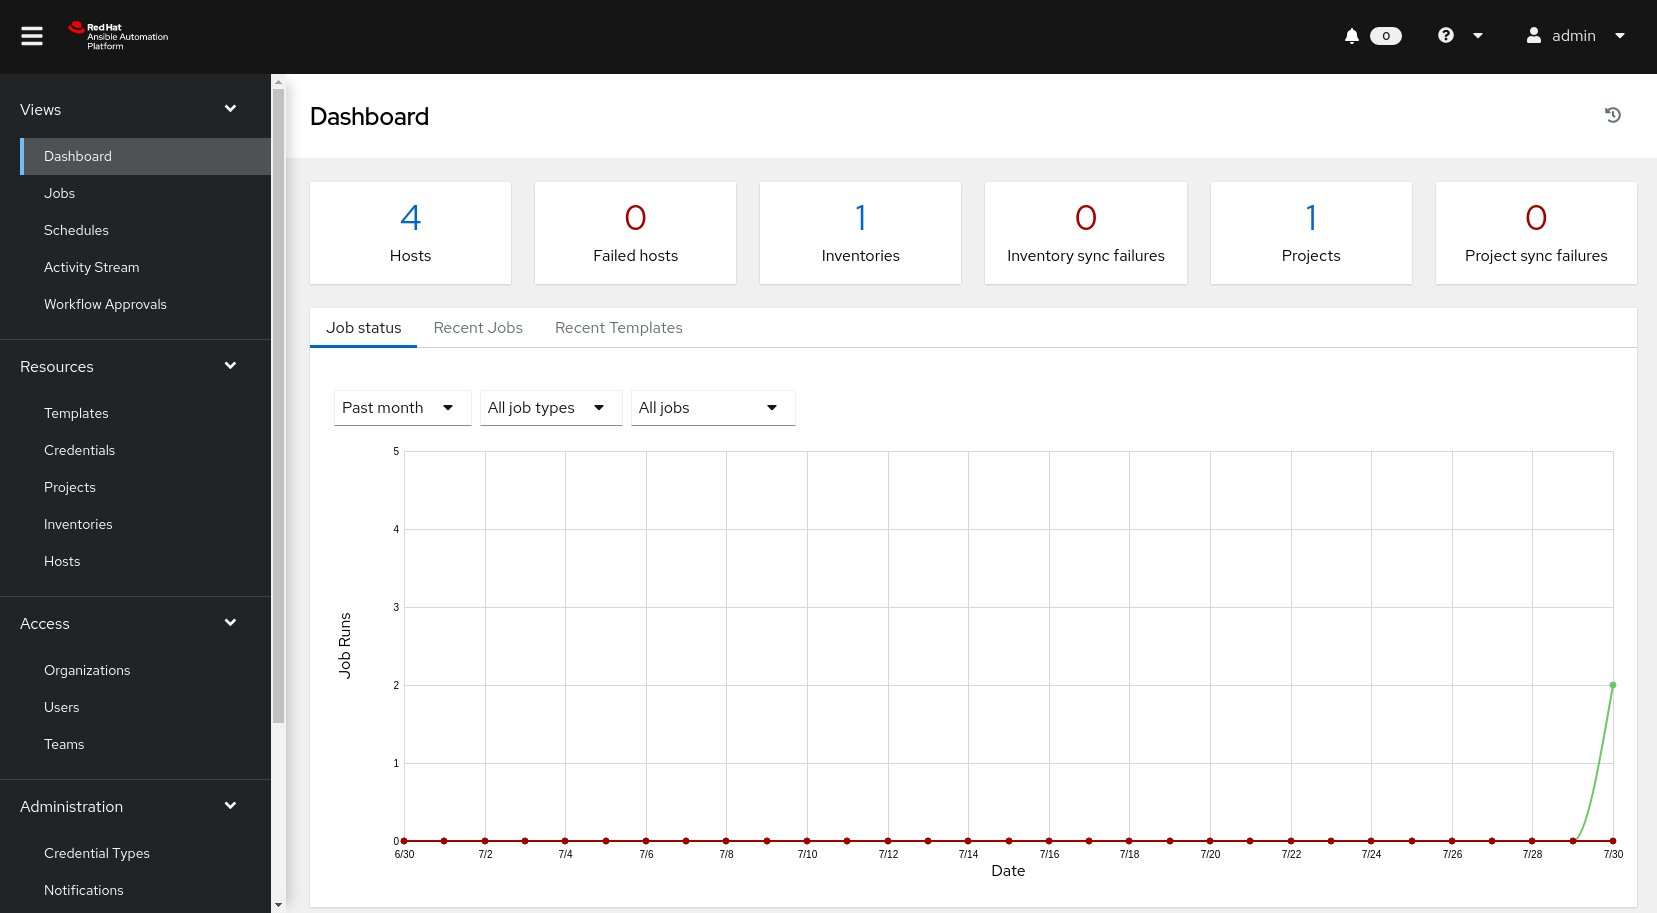
\includegraphics{images/02_controller_dashboard.jpg}
\caption{Ansible automation controller dashboard}
\end{figure}

\hypertarget{concepts}{%
\subsubsection{Concepts}\label{concepts}}

Before we dive further into using Ansible automation controller, you
should get familiar with some concepts and naming conventions.

\hypertarget{projects}{%
\paragraph{Projects}\label{projects}}

Projects are logical collections of Ansible playbooks in Ansible
automation controller. These playbooks either reside on the Ansible
automation controller instance, or in a source code version control
system supported by automation controller.

\hypertarget{inventories}{%
\paragraph{Inventories}\label{inventories}}

An Inventory is a collection of hosts against which jobs may be
launched, the same as an Ansible inventory file. Inventories are divided
into groups and these groups contain the actual hosts. Groups may be
populated manually, by entering host names into automation controller,
from one of Ansible Automation controller's supported cloud providers or
through dynamic inventory scripts.

\hypertarget{credentials}{%
\paragraph{Credentials}\label{credentials}}

Credentials are utilized by automation controller for authentication
when launching Jobs against machines, synchronizing with inventory
sources, and importing project content from a version control system.
Credential configuration can be found in the Settings.

automation controller credentials are imported and stored encrypted in
automation controller, and are not retrievable in plain text on the
command line by any user. You can grant users and teams the ability to
use these credentials, without actually exposing the credential to the
user.

\hypertarget{templates}{%
\paragraph{Templates}\label{templates}}

A job template is a definition and set of parameters for running an
Ansible job. Job templates are useful to execute the same job many
times. Job templates also encourage the reuse of Ansible playbook
content and collaboration between teams. To execute a job, automation
Controller requires that you first create a job template.

\hypertarget{jobs}{%
\paragraph{Jobs}\label{jobs}}

A job is basically an instance of automation controller launching an
Ansible playbook against an inventory of hosts.

\hypertarget{workshop-exercise---inventories-credentials-and-ad-hoc-commands}{%
\section{Workshop Exercise - Inventories, credentials and ad hoc
commands}\label{workshop-exercise---inventories-credentials-and-ad-hoc-commands}}

\hypertarget{objective}{%
\subsection{Objective}\label{objective}}

Explore and understand the lab environment. This exercise will cover

\begin{itemize}
\item
  Locating and understanding:

  \begin{itemize}
  \tightlist
  \item
    Ansible Automation Controller
    \href{https://docs.ansible.com/automation-controller/latest/html/userguide/inventories.html}{\textbf{Inventories}}
  \item
    Ansible Automation Controller
    \href{https://docs.ansible.com/automation-controller/latest/html/userguide/credentials.html}{\textbf{Credentials}}
  \end{itemize}
\item
  Running ad hoc commands via the Ansible Automation Controller web UI
\end{itemize}

\hypertarget{guide}{%
\subsection{Guide}\label{guide}}

\hypertarget{examine-an-inventory}{%
\subsubsection{Examine an Inventory}\label{examine-an-inventory}}

The first thing we need is an inventory of your managed hosts. This is
the equivalent of an inventory file in command-line Ansible. There is a
lot more to it (like dynamic inventories) but let's start with the
basics.

\begin{itemize}
\tightlist
\item
  You should already have the web UI open, if not: Point your browser to
  \texttt{https://10.3.48.100}. The password will be provided by the instructor.
\end{itemize}

There will be one inventory, the \textbf{[USER] Inventory}. Click the
\textbf{[USER] Inventory} then click the \textbf{Hosts} button

The inventory information at
\texttt{\textasciitilde{}/hosts} was pre-loaded into the
Ansible Automation controller Inventory as part of the provisioning
process.

\begin{Shaded}
\begin{Highlighting}[]
\ExtensionTok{$}\NormalTok{ cat \textasciitilde{}/hosts}
\ExtensionTok{[web]}
\ExtensionTok{node}\NormalTok{ ansible\_host=10.3.48.101 ansible\_user=s1}

\ExtensionTok{[control]}
\ExtensionTok{controller}\NormalTok{ ansible\_host=10.3.48.100 ansible\_user=s1}
\end{Highlighting}
\end{Shaded}

\begin{quote}
\textbf{Warning}

In your inventory the IP addresses will be different.
\end{quote}

\hypertarget{examine-machine-credentials}{%
\subsubsection{Examine Machine
Credentials}\label{examine-machine-credentials}}

Now we will examine the credentials to access our managed hosts from
Automation controller. As part of the provisioning process for this
Ansible Workshop the \textbf{[USER] Credential} has already been
setup.

In the \textbf{Resources} menu choose \textbf{Credentials}. Now click on
the \textbf{[USER] Credential}.

Note the following information:
\begin{itemize}
        \tightlist
    \item \textbf{Credential Type}: Machine- Machine credentials define ssh and user-level privilege
escalation access for playbooks. They are used when submitting jobs to
run playbooks on a remote host.
\item \textbf{Username}: matches our command-line Ansible inventory username for
the other Linux nodes
\item \textbf{SSH Private Key}: Encrypted - take note that you can't actually examine the SSH private
key once someone hands it over to Ansible Automation controller
\end{itemize}

\hypertarget{run-ad-hoc-commands}{%
\subsubsection{Run Ad Hoc commands}\label{run-ad-hoc-commands}}

It is possible to run run ad hoc commands from Ansible Automation
controller as well.

\begin{itemize}
\item
  In the webUI go to \textbf{Resources → Inventories → [USER]
  Inventory}
\item
  Click the \textbf{Hosts} tab to change into the hosts view and select
  the \texttt{node} host by ticking the box to the left of the host entry.
\item
  Click \textbf{Run Command} button. In the next screen you have to
  specify the ad hoc command.
\end{itemize}

Within the \textbf{Details} window, select \textbf{Module} \texttt{ping}
and click \textbf{Next}.

Within the \textbf{Execution Environment} window, select \textbf{Default
execution environment} and click \textbf{Next}.

Within the \textbf{Machine Credential} window, select \textbf{[USER]
Credentials} and click \textbf{Launch}.

\begin{quote}
\textbf{Tip}

The output of the results is displayed once the command has completed.
\end{quote}

The simple \textbf{ping} module doesn't need options. For other modules
you need to supply the command to run as an argument. Try the
\textbf{command} module to find the userid of the executing user using
an ad hoc command.

\begin{itemize}
\item
    In the web UI go to \textbf{Resources → Inventories → [USER]
  Inventory}
\item
  Click the \textbf{Hosts} tab to change into the hosts view and select
  the \texttt{node} host by ticking the box to the left of the host entry.
\item
  Click \textbf{Run Command} button. In the next screen you have to
  specify the ad hoc command.
\end{itemize}

Within the \textbf{Details} window, select \textbf{Module}
\texttt{command}, in \textbf{Arguments} type \texttt{id} and click
\textbf{Next}.

Within the \textbf{Execution Environment} window, select \textbf{Default
execution environment} and click \textbf{Next}.

Within the \textbf{Machine Credential} window, select \textbf{[USER]
Credentials} and click \textbf{Launch}.

\begin{quote}
\textbf{Tip}

After choosing the module to run, Ansible Automation Controller will
provide a link to the docs page for the module when clicking the
question mark next to ``Arguments''. This is handy, give it a try.
\end{quote}

How about trying to get some secret information from the system? Try to
print out \emph{/etc/shadow}.

\begin{itemize}
\item
    In the web UI go to \textbf{Resources → Inventories → [USER]
  Inventory}
\item
  Click the \textbf{Hosts} tab to change into the hosts view and select
  the \texttt{node} host by ticking the box to the left of the host entry.
\item
  Click \textbf{Run Command} button. In the next screen you have to
  specify the ad hoc command.
\end{itemize}

Within the \textbf{Details} window, select \textbf{Module}
\texttt{command}, in \textbf{Arguments} type \texttt{cat\ /etc/shadow}
and click \textbf{Next}.

Within the \textbf{Execution Environment} window, select \textbf{Default
execution environment} and click \textbf{Next}.

Within the \textbf{Machine Credential} window, select \textbf{[USER]
Credentials} and click \textbf{Launch}.

\begin{quote}
\textbf{Warning}

\textbf{Expect an error!}
\end{quote}

Oops, the last one didn't went well, all red.

Re-run the last ad hoc command but this time check the checkbox labeled
\textbf{Enable privilege escalation}.

As you see, this time it worked. For tasks that have to run as
\texttt{root} you need to escalate the privileges. This is the same as
the \textbf{become: True} used in your Ansible Playbooks.

\hypertarget{challenge-lab-ad-hoc-commands}{%
\subsubsection{Challenge Lab: Ad Hoc
Commands}\label{challenge-lab-ad-hoc-commands}}

Okay, a small challenge: Run an ad hoc to make sure the package ``tmux''
is installed on all hosts. If unsure, consult the documentation either
via the web UI as shown above or by running
\texttt{{[}ansible@controller\ \textasciitilde{}{]}\$\ ansible-doc\ yum}
on your Automation controller control host.

\begin{quote}
\textbf{Warning}

\textbf{Solution below!}
\end{quote}

\begin{itemize}
\item
    In the web UI go to \textbf{Resources → Inventories → [USER]
  Inventory}
\item
  Click the \textbf{Hosts} tab to change into the hosts view and select
  the \texttt{node} host by ticking the box to the left of the host entry.
\item
  Click \textbf{Run Command} button. In the next screen you have to
  specify the ad hoc command.
\end{itemize}

Within the \textbf{Details} window, select \textbf{Module} \texttt{yum},
in \textbf{Arguments} type \texttt{name=tmux}, check \textbf{Enable
privilege escalation} and click \textbf{Next}.

Within the \textbf{Execution Environment} window, select \textbf{Default
execution environment} and click \textbf{Next}.

Within the \textbf{Machine Credential} window, select \textbf{[USER]
Credentials} and click \textbf{Launch}.

\begin{quote}
\textbf{Tip}

Notice how the package was instaled via the ``CHANGED'' output. If you
run the ad hoc command a second time, the output will mention
``SUCCESS'' and inform you via the message parameter that there is
nothing to do.
\end{quote}

\hypertarget{workshop-exercise---projects-job-templates}{%
\section{Workshop Exercise - Projects \& Job
Templates}\label{workshop-exercise---projects-job-templates}}

\hypertarget{objective}{%
\subsection{Objective}\label{objective}}

An Ansible automation controller \textbf{Project} is a logical
collection of Ansible playbooks. You can manage your playbooks by
placing them into a source code management (SCM) system supported by
automation controller such as Git or Subversion.

This exercise covers:

\begin{itemize}
\tightlist
\item
  Understanding and using an Ansible automation controller Project
\item
  Using Ansible playbooks kept in a Git repository.
\item
  Creating and using an Ansible Job Template
\end{itemize}

\hypertarget{guide}{%
\subsection{Guide}\label{guide}}

\hypertarget{setup-git-repository}{%
\subsubsection{Setup Git Repository}\label{setup-git-repository}}

For this demonstration we will use playbooks stored in a Git repository:

\url{https://github.com/ansible/workshop-examples}

A playbook to install the Apache web server has already been committed
to the directory \textbf{rhel/apache}, \texttt{apache\_install.yml}:

\begin{Shaded}
\begin{Highlighting}[]
\PreprocessorTok{{-}{-}{-}}
\KeywordTok{{-}}\AttributeTok{ }\FunctionTok{name}\KeywordTok{:}\AttributeTok{ Apache server installed}
\AttributeTok{  }\FunctionTok{hosts}\KeywordTok{:}\AttributeTok{ web}

\AttributeTok{  }\FunctionTok{tasks}\KeywordTok{:}
\AttributeTok{  }\KeywordTok{{-}}\AttributeTok{ }\FunctionTok{name}\KeywordTok{:}\AttributeTok{ latest Apache version installed}
\AttributeTok{    }\FunctionTok{ansible.builtin.yum}\KeywordTok{:}
\AttributeTok{      }\FunctionTok{name}\KeywordTok{:}\AttributeTok{ httpd}
\AttributeTok{      }\FunctionTok{state}\KeywordTok{:}\AttributeTok{ latest}

\AttributeTok{  }\KeywordTok{{-}}\AttributeTok{ }\FunctionTok{name}\KeywordTok{:}\AttributeTok{ latest firewalld version installed}
\AttributeTok{    }\FunctionTok{ansible.builtin.yum}\KeywordTok{:}
\AttributeTok{      }\FunctionTok{name}\KeywordTok{:}\AttributeTok{ firewalld}
\AttributeTok{      }\FunctionTok{state}\KeywordTok{:}\AttributeTok{ latest}

\AttributeTok{  }\KeywordTok{{-}}\AttributeTok{ }\FunctionTok{name}\KeywordTok{:}\AttributeTok{ firewalld enabled and running}
\AttributeTok{    }\FunctionTok{ansible.builtin.service}\KeywordTok{:}
\AttributeTok{      }\FunctionTok{name}\KeywordTok{:}\AttributeTok{ firewalld}
\AttributeTok{      }\FunctionTok{enabled}\KeywordTok{:}\AttributeTok{ }\CharTok{true}
\AttributeTok{      }\FunctionTok{state}\KeywordTok{:}\AttributeTok{ started}

\AttributeTok{  }\KeywordTok{{-}}\AttributeTok{ }\FunctionTok{name}\KeywordTok{:}\AttributeTok{ firewalld permits http service}
\AttributeTok{    }\FunctionTok{ansible.builtin.firewalld}\KeywordTok{:}
\AttributeTok{      }\FunctionTok{service}\KeywordTok{:}\AttributeTok{ http}
\AttributeTok{      }\FunctionTok{permanent}\KeywordTok{:}\AttributeTok{ }\CharTok{true}
\AttributeTok{      }\FunctionTok{state}\KeywordTok{:}\AttributeTok{ enabled}
\AttributeTok{      }\FunctionTok{immediate}\KeywordTok{:}\AttributeTok{ }\CharTok{yes}

\AttributeTok{  }\KeywordTok{{-}}\AttributeTok{ }\FunctionTok{name}\KeywordTok{:}\AttributeTok{ Apache enabled and running}
\AttributeTok{    }\FunctionTok{ansible.builtin.service}\KeywordTok{:}
\AttributeTok{      }\FunctionTok{name}\KeywordTok{:}\AttributeTok{ httpd}
\AttributeTok{      }\FunctionTok{enabled}\KeywordTok{:}\AttributeTok{ }\CharTok{true}
\AttributeTok{      }\FunctionTok{state}\KeywordTok{:}\AttributeTok{ started}
\end{Highlighting}
\end{Shaded}

\begin{quote}
\textbf{Tip}

Note the difference to other playbooks you might have written! Most
importantly there is no \texttt{become} and \texttt{hosts} is set to
\texttt{all}.
\end{quote}

To configure and use this repository as a \textbf{Source Control
Management (SCM)} system in automation controller you have to create a
\textbf{Project} that uses the repository

\hypertarget{create-the-project}{%
\subsubsection{Create the Project}\label{create-the-project}}

\begin{itemize}
\tightlist
\item
  Go to \textbf{Resources → Projects} click the \textbf{Add} button.
  Fill in the form:

        \begin{itemize}
            \item \textbf{Name}: Workshop Project
            \item \textbf{Organization}: [USER]
            \item \textbf{Default Execution Environment}: Default execution environment
            \item \textbf{Source Control Credential Type}: Git
            \item Enter the URL into the \textbf{Project configuration}
            \item \textbf{Source Control URL}: https://github.com/ansible/workshop-examples.git
            \item \textbf{Options}: Select Clean, Delete, Update Revision on Launch to request a fresh copy
of the repository and to update the repository when launching a job.

\end{itemize}
\item
  Click \textbf{SAVE}
\end{itemize}

The new project will be synced automatically after creation. But you can
also do this manually: Sync the Project again with the Git repository by
going to the \textbf{Projects} view and clicking the circular arrow
\textbf{Sync Project} icon to the right of the Project.

After starting the sync job, go to the \textbf{Jobs} view: there is a
new job for the update of the Git repository.

\hypertarget{create-a-job-template-and-run-a-job}{%
\subsubsection{Create a Job Template and Run a
Job}\label{create-a-job-template-and-run-a-job}}

A job template is a definition and set of parameters for running an
Ansible job. Job templates are useful to execute the same job many
times. So before running an Ansible \textbf{Job} from automation
controller you must create a \textbf{Job Template} that pulls together:

\begin{itemize}
\item
  \textbf{Inventory}: On what hosts should the job run?
\item
  \textbf{Credentials} What credentials are needed to log into the
  hosts?
\item
  \textbf{Project}: Where is the playbook?
\item
  \textbf{What} playbook to use?
\end{itemize}

Okay, let's just do that: Go to the \textbf{Resources -\textgreater{}
Templates} view, click the \textbf{Add} button and choose \textbf{Add
job template}.

\begin{quote}
\textbf{Tip}

Remember that you can often click on magnfying glasses to get an
overview of options to pick to fill in fields.
\end{quote}
\begin{itemize}
\tightlist
    \item \textbf{Name}: Install Apache
    \item \textbf{Job Type}: Run
    \item \textbf{Inventory}: [USER] Inventory
    \item \textbf{Project}: Workshop Project
    \item \textbf{Execution Environment}: Default execution environment
    \item \textbf{Playbook}: rhel/apache/apache\_install.yml
    \item \textbf{Credentials}: [USER] Credential
    \item \textbf{Limit}: web
    \item tasks need to run as root so check \textbf{Privilege Escalation}
\end{itemize}

\begin{itemize}
\tightlist
\item
  Click \textbf{Save}
\end{itemize}

You can start the job by directly clicking the blue \textbf{Launch}
button, or by clicking on the rocket in the Job Templates overview.
After launching the Job Template, you are automatically brought to the
job overview where you can follow the playbook execution in real time:

Job Details 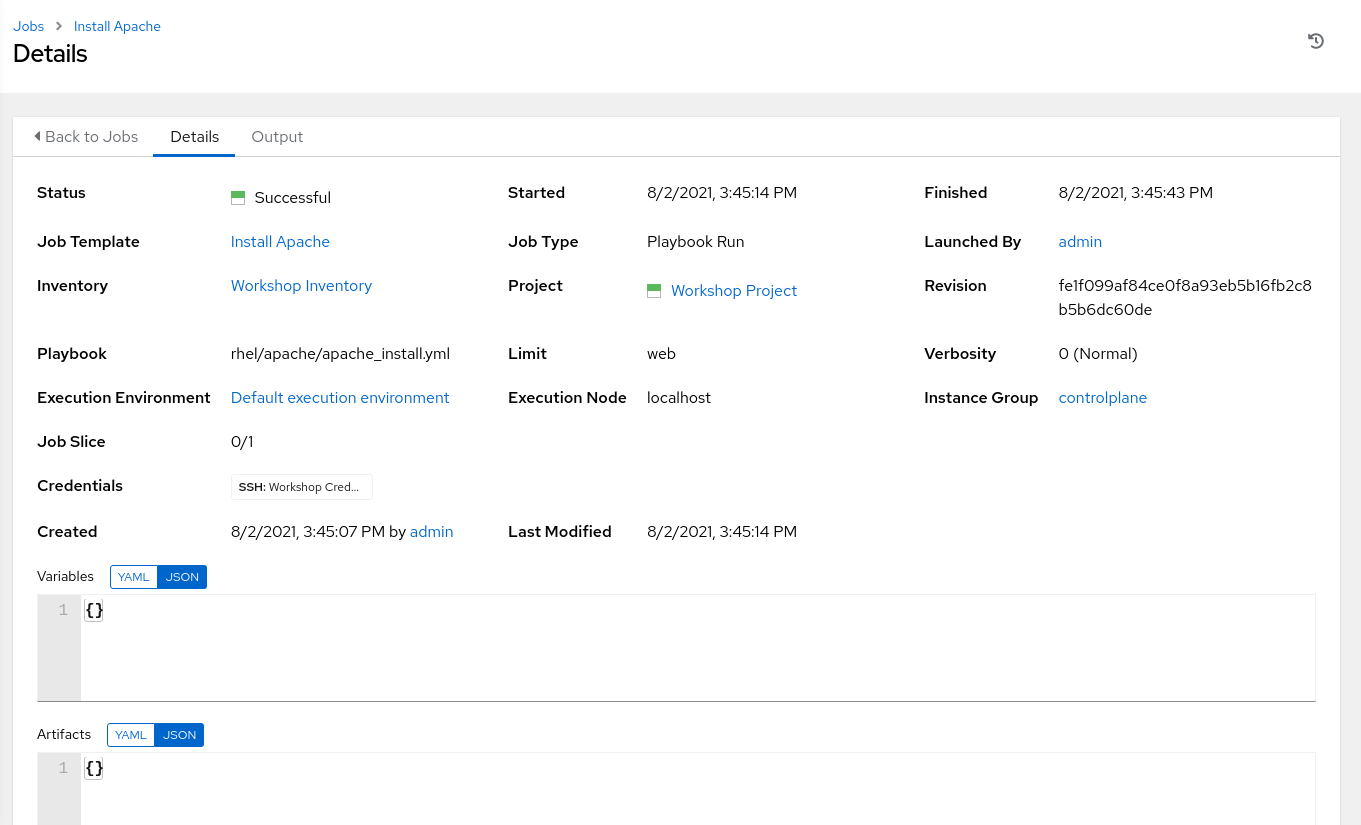
\includegraphics{images/02_job_details.png}

Job Run 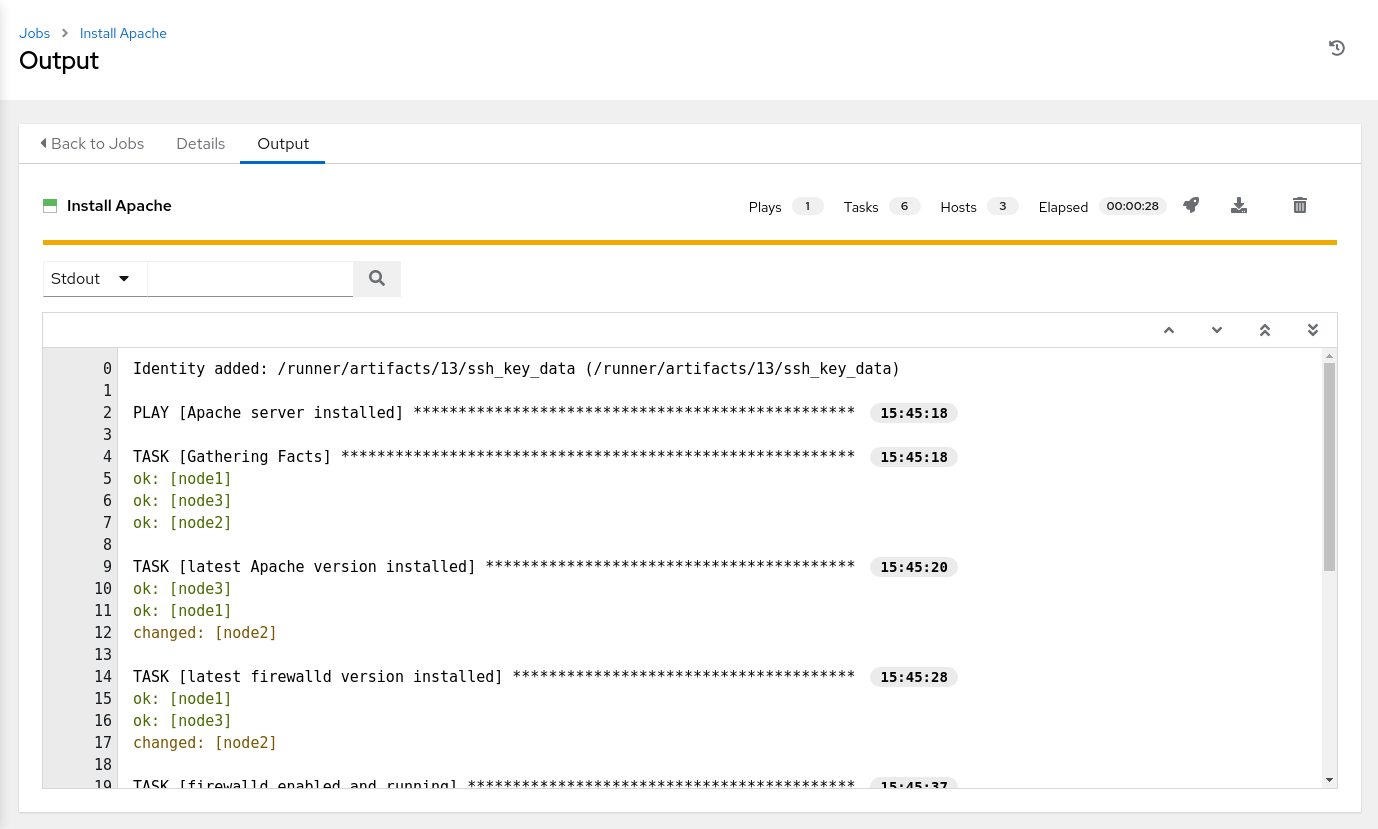
\includegraphics{images/02_job_run.png}

Since this might take some time, have a closer look at all the details
provided:

\begin{itemize}
\item
  All details of the job template like inventory, project, credentials
  and playbook are shown.
\item
  Additionally, the actual revision of the playbook is recorded here -
  this makes it easier to analyse job runs later on.
\item
  Also the time of execution with start and end time is recorded, giving
  you an idea of how long a job execution actually was.
\item
  Selecting \textbf{Output} shows the output of the running playbook.
  Click on a node underneath a task and see that detailed information
  are provided for each task of each node.
\end{itemize}

After the Job has finished go to the main \textbf{Jobs} view: All jobs
are listed here, you should see directly before the Playbook run an
Source Control Update was started. This is the Git update we configured
for the \textbf{Project} on launch!

\hypertarget{challenge-lab-check-the-result}{%
\subsubsection{Challenge Lab: Check the
Result}\label{challenge-lab-check-the-result}}

Time for a little challenge:

\begin{itemize}
\tightlist
\item
  Use an ad hoc command on both hosts to make sure Apache has been
  installed and is running.
\end{itemize}

You have already been through all the steps needed, so try this for
yourself.

\begin{quote}
\textbf{Tip}

What about \texttt{systemctl\ status\ httpd}?
\end{quote}

\begin{quote}
\textbf{Warning}

\textbf{Solution Below}
\end{quote}

\begin{itemize}
\item
  Go to \textbf{Resources → Inventories} → \textbf{[USER] Inventory}
\item
  In the \textbf{Hosts} view select \texttt{node} and click \textbf{Run Command}
\end{itemize}

Within the \textbf{Details} window, select \textbf{Module}
\texttt{command}, in \textbf{Arguments} type
\texttt{systemctl\ status\ httpd} and click \textbf{Next}.

Within the \textbf{Execution Environment} window, select \textbf{Default
execution environment} and click \textbf{Next}.

Within the \textbf{Machine Credential} window, select \textbf{[USER]
Credential} and click \textbf{Launch}.

\begin{quote}
\textbf{Tip}

The output of the results is displayed once the command has completed.
\end{quote}

\hypertarget{workshop-exercise---role-based-access-control}{%
\section{Workshop Exercise - Role-based access
control}\label{workshop-exercise---role-based-access-control}}

\hypertarget{objective}{%
\subsection{Objective}\label{objective}}

You have already learned how Ansible automation controller separates
credentials from users. Another advantage of Ansible automation
controller is the user and group rights management. This exercise
demonstrates Role Based Access Control (RBAC)

\hypertarget{guide}{%
\subsection{Guide}\label{guide}}

\hypertarget{ansible-automation-controller-users}{%
\subsubsection{Ansible automation controller
users}\label{ansible-automation-controller-users}}

There are three types of automation controller users:

\begin{itemize}
\item
  \textbf{Normal User}: Have read and write access limited to the
  inventory and projects for which that user has been granted the
  appropriate roles and privileges.
\item
  \textbf{System Auditor}: Auditors implicitly inherit the read-only
  capability for all objects within the automation controller
  environment.
\item
  \textbf{System Administrator}: Has admin, read, and write privileges
  over the entire automation controller installation.
\end{itemize}

Let's create a user:

\begin{itemize}
\item
  In the automation controller menu under \textbf{Access} click
  \textbf{Users}
\item
  Click the \textbf{Add} button
\item
  Fill in the values for the new user:

        \begin{itemize}
            \item \textbf{Username}: [USER]-wweb
            \item \textbf{Password}: ansible
            \item \textbf{Confirm Password}: ansible
            \item \textbf{Organization}: [USER]
            \item \textbf{User Type}: Normal User
        \end{itemize}

\item
  Click \textbf{Save}
\end{itemize}

\hypertarget{ansible-automation-controller-teams}{%
\subsubsection{Ansible automation controller
teams}\label{ansible-automation-controller-teams}}

A Team is a subdivision of an organization with associated users,
projects, credentials, and permissions. Teams provide a means to
implement role-based access control schemes and delegate
responsibilities across organizations. For instance, permissions may be
granted to a whole Team rather than each user on the Team.

Create a Team:

\begin{itemize}
\item
  In the menu go to \textbf{Access → Teams}
\item
  Click the \textbf{Add} button and create a team named
  \texttt{[USER] Web\ Content} within the \texttt{[USER]} Organization.
\item
  Click \textbf{Save}
\end{itemize}

Add a user to the team:

\begin{itemize}
\item
  Click on the team \texttt{[USER] Web\ Content} and click the \textbf{Access}
  tab and click \textbf{Add}.
\item
  Within the \textbf{Select a Resource Type} window, click on the
  \textbf{Users} resource type and click \textbf{Next}.
\item
  Within the \textbf{Select Items from List}, select the checkbox next
  to the \texttt{[USER]-wweb} user and click \textbf{Next}.
\item
  Within the \textbf{Select Roles to Apply}, select \textbf{Member} as
  the role to apply to the \texttt{[USER]-wweb} user.
\end{itemize}

Click \textbf{Save}.

Permissions allow to read, modify, and administer projects, inventories,
and other automation controller elements. Permissions can be set for
different resources.

\hypertarget{granting-permissions}{%
\subsubsection{Granting permissions}\label{granting-permissions}}

To allow users or teams to actually do something, you have to set
permissions. The user \textbf{[USER]-wweb} should only be allowed to modify
content of the assigned webservers.

Add the permission to use the \texttt{Create\ index.html} template:

\begin{itemize}
\item
  Within \textbf{Resources} -\textgreater{} \textbf{Templates}, select
  \texttt{Create\ index.html}.
\item
  Select \textbf{Access} tab from the menu and click \textbf{Add}.
\item
  Within the \textbf{Select a Resource Type} window, click on the
  \textbf{Users} resource type and click \textbf{Next}.
\item
  Within the \textbf{Select Items from List}, select the checkbox next
  to the \texttt{[USER]-wweb} user and click \textbf{Next}.
\item
  Within the \textbf{Select Roles to Apply}, select \textbf{Read} and
  \textbf{Execute} as the roles to apply to the \texttt{[USER]-wweb} user.
\item
  Click \textbf{Save}
\end{itemize}

\hypertarget{test-permissions}{%
\subsubsection{Test permissions}\label{test-permissions}}

Now log out of automation controller's web UI and in again as the
\textbf{[USER]-wweb} user.

\begin{itemize}
\item
  Go to the \textbf{Templates} view, you should notice for wweb only the
  \texttt{Create\ \ \ index.html} template is listed. He is allowed to
  view and launch, but not to edit the Template (no Edit button
  available).
\item
  Run the Job Template by clicking the rocket icon. Enter the values for
  the survey questions and launch the job.
\item
  In the following \textbf{Jobs} view have a good look around, note that
  there where changes to the host (as expected).
\end{itemize}

Check the result: execute \texttt{curl} again on the control host to
pull the content of the webserver on \texttt{node}:

\begin{Shaded}
\begin{Highlighting}[]
\CommentTok{\#\textgreater{} curl http://10.3.48.[100+PARTICIPANT\_ID]}
\end{Highlighting}
\end{Shaded}

Just recall what you have just done: You enabled a restricted user to
run an Ansible playbook

\begin{itemize}
\item
  Without having access to the credentials
\item
  Without being able to change the playbook itself
\item
  But with the ability to change variables you predefined!
\end{itemize}

Effectively you provided the power to execute automation to another user
without handing out your credentials or giving the user the ability to
change the automation code. And yet, at the same time the user can still
modify things based on the surveys you created.

This capability is one of the main strengths of Ansible automation
controller!

\chapter{Ansible - advanced}
\hypertarget{conditionals-handlers-and-loops}{%
\section{Conditionals, Handlers and
Loops}\label{conditionals-handlers-and-loops}}


\hypertarget{objective}{%
\subsection{Objective}\label{objective}}

Three foundational Ansible features are:

\begin{itemize}
\tightlist
\item
  \href{https://docs.ansible.com/ansible/latest/user_guide/playbooks_conditionals.html}{Conditionals}
\item
  \href{https://docs.ansible.com/ansible/latest/user_guide/playbooks_intro.html\#handlers-running-operations-on-change}{Handlers}
\item
  \href{https://docs.ansible.com/ansible/latest/user_guide/playbooks_loops.html}{Loops}
\end{itemize}

\hypertarget{guide}{%
\subsection{Guide}\label{guide}}

\hypertarget{step-1---conditionals}{%
\subsubsection{Step 1 - Conditionals}\label{step-1---conditionals}}

Ansible can use conditionals to execute tasks or plays when certain
conditions are met.

To implement a conditional, the \texttt{when} statement must be used,
followed by the condition to test. The condition is expressed using one
of the available operators like e.g.~for comparison:

\begin{longtable}[]{@{}
  >{\raggedright\arraybackslash}p{(\columnwidth - 2\tabcolsep) * \real{0.0541}}
  >{\raggedright\arraybackslash}p{(\columnwidth - 2\tabcolsep) * \real{0.9459}}@{}}
\toprule\noalign{}
\endhead
\bottomrule\noalign{}
\endlastfoot
== & Compares two objects for equality. \\
!= & Compares two objects for inequality. \\
\textgreater{} & true if the left hand side is greater than the right
hand side. \\
\textgreater= & true if the left hand side is greater or equal to the
right hand side. \\
\textless{} & true if the left hand side is lower than the right hand
side. \\
\textless= & true if the left hand side is lower or equal to the right
hand side. \\
\end{longtable}

For more on this, please refer to the documentation:
\url{http://jinja.pocoo.org/docs/2.10/templates/}

As an example you would like to install an FTP server, but only on hosts
that are in the ``ftpserver'' inventory group.

To do that, first edit the inventory to add another group, and place
\texttt{node} in it. The section to add looks like this:

\begin{Shaded}
\begin{Highlighting}[]
\KeywordTok{[ftpserver]}
\DataTypeTok{node}
\end{Highlighting}
\end{Shaded}

Edit the inventory \texttt{\textasciitilde{}/hosts} to
add those lines. When you are done, it will look similar to the
following listing:

\begin{quote}
\textbf{Tip}

The ansible\_host variable only needs to be specified once for a node.
When adding a node to other groups, you do not need to specify the
variable again.
\end{quote}

\textbf{Important} Do not copy/paste the example below. Just edit the
file to add the above lines.

\begin{Shaded}
\begin{Highlighting}[]
\KeywordTok{[web]}
\DataTypeTok{node ansible\_host}\OtherTok{=}\StringTok{xx.xx.xx.xx} \DataTypeTok{ansible\_user}\OtherTok{=}\StringTok{[USER]}

\KeywordTok{[ftpserver]}
\DataTypeTok{node}

\KeywordTok{[control]}
\DataTypeTok{controller ansible\_host}\OtherTok{=}\StringTok{xx.xx.xx.xx} \DataTypeTok{ansible\_user}\OtherTok{=}\StringTok{[USER]}
\end{Highlighting}
\end{Shaded}

Next create the file \texttt{ftpserver.yml} on your control host in the
\texttt{\textasciitilde{}/ansible-files/} directory:

\begin{Shaded}
\begin{Highlighting}[]
\PreprocessorTok{{-}{-}{-}}
\KeywordTok{{-}}\AttributeTok{ }\FunctionTok{name}\KeywordTok{:}\AttributeTok{ Install vsftpd on ftpservers}
\AttributeTok{  }\FunctionTok{hosts}\KeywordTok{:}\AttributeTok{ all}
\AttributeTok{  }\FunctionTok{become}\KeywordTok{:}\AttributeTok{ }\CharTok{True}
\AttributeTok{  }\FunctionTok{tasks}\KeywordTok{:}
\AttributeTok{    }\KeywordTok{{-}}\AttributeTok{ }\FunctionTok{name}\KeywordTok{:}\AttributeTok{ Install FTP server when host in ftpserver group}
\AttributeTok{      }\FunctionTok{ansible.builtin.yum}\KeywordTok{:}
\AttributeTok{        }\FunctionTok{name}\KeywordTok{:}\AttributeTok{ vsftpd}
\AttributeTok{        }\FunctionTok{state}\KeywordTok{:}\AttributeTok{ latest}
\AttributeTok{      }\FunctionTok{when}\KeywordTok{:}\AttributeTok{ inventory\_hostname in groups["ftpserver"]}
\end{Highlighting}
\end{Shaded}

\begin{quote}
\textbf{Tip}

By now you should know how to run Ansible Playbooks, we'll start to be
less verbose in this guide. Go create and run it. :-)
\end{quote}

Run it and examine the output. The expected outcome: The task is skipped
on the ansible host (your control host) because they
are not in the ftpserver group in your inventory file.

\begin{Shaded}
\begin{Highlighting}[]
\ExtensionTok{TASK}\NormalTok{ [Install FTP server when host in ftpserver group] }\PreprocessorTok{**************}
\ExtensionTok{skipping:} \PreprocessorTok{[}\SpecialStringTok{controller}\PreprocessorTok{]}
\ExtensionTok{changed:} \PreprocessorTok{[}\SpecialStringTok{node}\PreprocessorTok{]}
\end{Highlighting}
\end{Shaded}

\hypertarget{step-2---handlers}{%
\subsubsection{Step 2 - Handlers}\label{step-2---handlers}}

Sometimes when a task does make a change to the system, an additional
task or tasks may need to be run. For example, a change to a service's
configuration file may then require that the service be restarted so
that the changed configuration takes effect.

Here Ansible's handlers come into play. Handlers can be seen as inactive
tasks that only get triggered when explicitly invoked using the
``notify'' statement. Read more about them in the
\href{http://docs.ansible.com/ansible/latest/playbooks_intro.html\#handlers-running-operations-on-change}{Ansible
Handlers} documentation.

As a an example, let's write a playbook that:

\begin{itemize}
\tightlist
\item
  manages Apache's configuration file
  \texttt{/etc/httpd/conf/httpd.conf} on all hosts in the \texttt{web}
  group
\item
  restarts Apache when the file has changed
\end{itemize}

First we need the file Ansible will deploy, let's just take the one from
node1. Remember to replace the IP address shown in the listing below
with the IP address from your individual \texttt{node1}.

\begin{Shaded}
\begin{Highlighting}[]
\ExtensionTok{[student@controller}\NormalTok{ ansible{-}files]$ scp 10.3.48.[100+PARTICIPANT\_ID]:/etc/httpd/conf/httpd.conf \\}
\ExtensionTok{\textasciitilde{}/ansible{-}files/files/httpd.conf}
\end{Highlighting}
\end{Shaded}

Next, create the Playbook \texttt{httpd\_conf.yml}. Make sure that you
are in the directory \texttt{\textasciitilde{}/ansible-files}.

\begin{Shaded}
\begin{Highlighting}[]
\PreprocessorTok{{-}{-}{-}}
\KeywordTok{{-}}\AttributeTok{ }\FunctionTok{name}\KeywordTok{:}\AttributeTok{ Manage httpd.conf}
\AttributeTok{  }\FunctionTok{hosts}\KeywordTok{:}\AttributeTok{ web}
\AttributeTok{  }\FunctionTok{become}\KeywordTok{:}\AttributeTok{ }\CharTok{True}
\AttributeTok{  }\FunctionTok{tasks}\KeywordTok{:}
\AttributeTok{    }\KeywordTok{{-}}\AttributeTok{ }\FunctionTok{name}\KeywordTok{:}\AttributeTok{ Copy Apache configuration file}
\AttributeTok{      }\FunctionTok{ansible.builtin.copy}\KeywordTok{:}
\AttributeTok{        }\FunctionTok{src}\KeywordTok{:}\AttributeTok{ httpd.conf}
\AttributeTok{        }\FunctionTok{dest}\KeywordTok{:}\AttributeTok{ /etc/httpd/conf/}
\AttributeTok{        }\FunctionTok{mode}\KeywordTok{:}\AttributeTok{ }\StringTok{\textquotesingle{}644\textquotesingle{}}
\AttributeTok{      }\FunctionTok{notify}\KeywordTok{:}
\AttributeTok{        }\KeywordTok{{-}}\AttributeTok{ Restart\_apache}
\AttributeTok{    }\KeywordTok{{-}}\AttributeTok{ }\FunctionTok{name}\KeywordTok{:}\AttributeTok{ Open firewall port}
\AttributeTok{      }\FunctionTok{ansible.posix.firewalld}\KeywordTok{:}
\AttributeTok{        }\FunctionTok{port}\KeywordTok{:}\AttributeTok{ 8080/tcp}
\AttributeTok{        }\FunctionTok{immediate}\KeywordTok{:}\CharTok{ True}
\AttributeTok{        }\FunctionTok{permanent}\KeywordTok{:}\CharTok{ True}
\AttributeTok{        }\FunctionTok{state}\KeywordTok{:}\AttributeTok{ enabled}
\AttributeTok{  }\FunctionTok{handlers}\KeywordTok{:}
\AttributeTok{    }\KeywordTok{{-}}\AttributeTok{ }\FunctionTok{name}\KeywordTok{:}\AttributeTok{ Restart\_apache}
\AttributeTok{      }\FunctionTok{ansible.builtin.service}\KeywordTok{:}
\AttributeTok{        }\FunctionTok{name}\KeywordTok{:}\AttributeTok{ httpd}
\AttributeTok{        }\FunctionTok{state}\KeywordTok{:}\AttributeTok{ restarted}
\end{Highlighting}
\end{Shaded}

So what's new here?

\begin{itemize}
\tightlist
\item
  The ``notify'' section calls the handler only when the copy task
  actually changes the file. That way the service is only restarted if
  needed - and not each time the playbook is run.
\item
  The ``handlers'' section defines a task that is only run on
  notification.
\end{itemize}

Run the playbook. We didn't change anything in the file yet so there
should not be any \texttt{changed} lines in the output and of course the
handler shouldn't have fired.

\begin{itemize}
\tightlist
\item
  Now change the \texttt{Listen\ 80} line in
  \texttt{\textasciitilde{}/ansible-files/files/httpd.conf} to:
\end{itemize}

\begin{Shaded}
\begin{Highlighting}[]
\DataTypeTok{Listen 8080}
\end{Highlighting}
\end{Shaded}

\begin{itemize}
\item
  Run the playbook again. Now the Ansible's output should be a lot more
  interesting:

  \begin{itemize}
  \tightlist
  \item
    httpd.conf should have been copied over
  \item
    The handler should have restarted Apache
  \end{itemize}
\end{itemize}

Apache should now listen on port 8080. Easy enough to verify:

\begin{Shaded}
\begin{Highlighting}[]
\ExtensionTok{[student@controller}\NormalTok{ ansible{-}files]$ curl http://10.3.48.[100+PARTICIPANT\_ID]}
\ExtensionTok{curl:} \ExtensionTok{(7)} \ExtensionTok{Failed}\NormalTok{ to connect to 10.3.48.101 port 80: Connection refused}
\ExtensionTok{[student@controller}\NormalTok{ ansible{-}files]$ curl http://10.3.48.[100+PARTICIPANT\_ID]:8080}
\OperatorTok{\textless{}}\NormalTok{body}\OperatorTok{\textgreater{}}
\OperatorTok{  \textless{}}\NormalTok{h1}\OperatorTok{\textgreater{}}\NormalTok{Apache }\ExtensionTok{is}\NormalTok{ running fine}\OperatorTok{\textless{}}\NormalTok{/h1}\OperatorTok{\textgreater{}}
\OperatorTok{\textless{}}\NormalTok{/body}\OperatorTok{\textgreater{}}
\end{Highlighting}
\end{Shaded}

Leave the setting for listen on port 8080. We'll use this in a later
exercise.

\hypertarget{step-3---simple-loops}{%
\subsubsection{Step 3 - Simple Loops}\label{step-3---simple-loops}}

Loops enable us to repeat the same task over and over again. For
example, lets say you want to create multiple users. By using an Ansible
loop, you can do that in a single task. Loops can also iterate over more
than just basic lists. For example, if you have a list of users with
their coresponding group, loop can iterate over them as well. Find out
more about loops in the
\href{https://docs.ansible.com/ansible/latest/user_guide/playbooks_loops.html}{Ansible
Loops} documentation.

To show the loops feature we will generate three new users on
\texttt{node}. For that, create the file \texttt{loop\_users.yml} in
\texttt{\textasciitilde{}/ansible-files} on your control node as your
student user. We will use the \texttt{user} module to generate the user
accounts.

\begin{Shaded}
\begin{Highlighting}[]
\PreprocessorTok{{-}{-}{-}}
\KeywordTok{{-}}\AttributeTok{ }\FunctionTok{name}\KeywordTok{:}\AttributeTok{ Ensure users}
\AttributeTok{  }\FunctionTok{hosts}\KeywordTok{:}\AttributeTok{ node}
\AttributeTok{  }\FunctionTok{become}\KeywordTok{:}\AttributeTok{ }\CharTok{True}
\AttributeTok{  }\FunctionTok{tasks}\KeywordTok{:}
\AttributeTok{    }\KeywordTok{{-}}\AttributeTok{ }\FunctionTok{name}\KeywordTok{:}\AttributeTok{ Ensure three users are present}
\AttributeTok{      }\FunctionTok{ansible.builtin.user}\KeywordTok{:}
\AttributeTok{        }\FunctionTok{name}\KeywordTok{:}\AttributeTok{ }\StringTok{"\{\{ item \}\}"}
\AttributeTok{        }\FunctionTok{state}\KeywordTok{:}\AttributeTok{ present}
\AttributeTok{      }\FunctionTok{loop}\KeywordTok{:}
\AttributeTok{         }\KeywordTok{{-}}\AttributeTok{ dev\_user}
\AttributeTok{         }\KeywordTok{{-}}\AttributeTok{ qa\_user}
\AttributeTok{         }\KeywordTok{{-}}\AttributeTok{ prod\_user}
\end{Highlighting}
\end{Shaded}

Understand the playbook and the output:

\begin{itemize}
\tightlist
\item
  The names are not provided to the user module directly. Instead, there
  is only a variable called \texttt{\{\{\ item\ \}\}} for the parameter
  \texttt{name}.
\item
  The \texttt{loop} keyword lists the actual user names. Those replace
  the \texttt{\{\{\ item\ \}\}} during the actual execution of the
  playbook.
\item
  During execution the task is only listed once, but there are three
  changes listed underneath it.
\end{itemize}

\hypertarget{step-4---loops-over-hashes}{%
\subsubsection{Step 4 - Loops over
hashes}\label{step-4---loops-over-hashes}}

As mentioned loops can also be over lists of hashes. Imagine that the
users should be assigned to different additional groups:

\begin{Shaded}
\begin{Highlighting}[]
\KeywordTok{{-}}\AttributeTok{ }\FunctionTok{username}\KeywordTok{:}\AttributeTok{ dev\_user}
\AttributeTok{  }\FunctionTok{groups}\KeywordTok{:}\AttributeTok{ ftp}
\KeywordTok{{-}}\AttributeTok{ }\FunctionTok{username}\KeywordTok{:}\AttributeTok{ qa\_user}
\AttributeTok{  }\FunctionTok{groups}\KeywordTok{:}\AttributeTok{ ftp}
\KeywordTok{{-}}\AttributeTok{ }\FunctionTok{username}\KeywordTok{:}\AttributeTok{ prod\_user}
\AttributeTok{  }\FunctionTok{groups}\KeywordTok{:}\AttributeTok{ apache}
\end{Highlighting}
\end{Shaded}

The \texttt{user} module has the optional parameter \texttt{groups} to
list additional users. To reference items in a hash, the
\texttt{\{\{\ item\ \}\}} keyword needs to reference the subkey:
\texttt{\{\{\ item.groups\ \}\}} for example.

Let's rewrite the playbook to create the users with additional user
rights:

\begin{Shaded}
\begin{Highlighting}[]
\PreprocessorTok{{-}{-}{-}}
\KeywordTok{{-}}\AttributeTok{ }\FunctionTok{name}\KeywordTok{:}\AttributeTok{ Ensure users}
\AttributeTok{  }\FunctionTok{hosts}\KeywordTok{:}\AttributeTok{ node}
\AttributeTok{  }\FunctionTok{become}\KeywordTok{:}\AttributeTok{ }\CharTok{True}
\AttributeTok{  }\FunctionTok{tasks}\KeywordTok{:}
\AttributeTok{    }\KeywordTok{{-}}\AttributeTok{ }\FunctionTok{name}\KeywordTok{:}\AttributeTok{ Ensure three users are present}
\AttributeTok{      }\FunctionTok{ansible.builtin.user}\KeywordTok{:}
\AttributeTok{        }\FunctionTok{name}\KeywordTok{:}\AttributeTok{ }\StringTok{"\{\{ item.username \}\}"}
\AttributeTok{        }\FunctionTok{state}\KeywordTok{:}\AttributeTok{ present}
\AttributeTok{        }\FunctionTok{groups}\KeywordTok{:}\AttributeTok{ }\StringTok{"\{\{ item.groups \}\}"}
\AttributeTok{      }\FunctionTok{loop}\KeywordTok{:}
\AttributeTok{        }\KeywordTok{{-}}\AttributeTok{ }\KeywordTok{\{}\AttributeTok{ }\FunctionTok{username}\KeywordTok{:}\AttributeTok{ }\StringTok{\textquotesingle{}dev\_user\textquotesingle{}}\KeywordTok{,}\AttributeTok{ }\FunctionTok{groups}\KeywordTok{:}\AttributeTok{ }\StringTok{\textquotesingle{}ftp\textquotesingle{}}\AttributeTok{ }\KeywordTok{\}}
\AttributeTok{        }\KeywordTok{{-}}\AttributeTok{ }\KeywordTok{\{}\AttributeTok{ }\FunctionTok{username}\KeywordTok{:}\AttributeTok{ }\StringTok{\textquotesingle{}qa\_user\textquotesingle{}}\KeywordTok{,}\AttributeTok{ }\FunctionTok{groups}\KeywordTok{:}\AttributeTok{ }\StringTok{\textquotesingle{}ftp\textquotesingle{}}\AttributeTok{ }\KeywordTok{\}}
\AttributeTok{        }\KeywordTok{{-}}\AttributeTok{ }\KeywordTok{\{}\AttributeTok{ }\FunctionTok{username}\KeywordTok{:}\AttributeTok{ }\StringTok{\textquotesingle{}prod\_user\textquotesingle{}}\KeywordTok{,}\AttributeTok{ }\FunctionTok{groups}\KeywordTok{:}\AttributeTok{ }\StringTok{\textquotesingle{}apache\textquotesingle{}}\AttributeTok{ }\KeywordTok{\}}
\end{Highlighting}
\end{Shaded}

Check the output:

\begin{itemize}
\tightlist
\item
  Again the task is listed once, but three changes are listed. Each loop
  with its content is shown.
\end{itemize}

Verify that the user \texttt{dev\_user} was indeed created on
\texttt{node} using the following playbook:

\begin{Shaded}
\begin{Highlighting}[]
\PreprocessorTok{{-}{-}{-}}
\KeywordTok{{-}}\AttributeTok{ }\FunctionTok{name}\KeywordTok{:}\AttributeTok{ Get user ID}
\AttributeTok{  }\FunctionTok{hosts}\KeywordTok{:}\AttributeTok{ node}
\AttributeTok{  }\FunctionTok{vars}\KeywordTok{:}
\AttributeTok{    }\FunctionTok{myuser}\KeywordTok{:}\AttributeTok{ }\StringTok{"dev\_user"}
\AttributeTok{  }\FunctionTok{tasks}\KeywordTok{:}
\AttributeTok{    }\KeywordTok{{-}}\AttributeTok{ }\FunctionTok{name}\KeywordTok{:}\AttributeTok{ Get \{\{ myuser \}\} info}
\AttributeTok{      }\FunctionTok{ansible.builtin.getent}\KeywordTok{:}
\AttributeTok{        }\FunctionTok{database}\KeywordTok{:}\AttributeTok{ passwd}
\AttributeTok{        }\FunctionTok{key}\KeywordTok{:}\AttributeTok{ }\StringTok{"\{\{ myuser \}\}"}
\AttributeTok{    }\KeywordTok{{-}}\AttributeTok{ }\FunctionTok{ansible.builtin.debug}\KeywordTok{:}
\AttributeTok{        }\FunctionTok{msg}\KeywordTok{:}
\AttributeTok{          }\KeywordTok{{-}}\AttributeTok{ }\StringTok{"\{\{ myuser \}\} uid: \{\{ getent\_passwd[myuser].1 \}\}"}
\end{Highlighting}
\end{Shaded}

\begin{Shaded}
\begin{Highlighting}[]
\ExtensionTok{$}\NormalTok{ ansible{-}navigator run user\_id.yml }\AttributeTok{{-}m}\NormalTok{ stdout}

\ExtensionTok{PLAY}\NormalTok{ [Get user ID] }\PreprocessorTok{*************************************************************}

\ExtensionTok{TASK}\NormalTok{ [Gathering Facts] }\PreprocessorTok{*********************************************************}
\ExtensionTok{ok:} \PreprocessorTok{[}\SpecialStringTok{node}\PreprocessorTok{]}

\ExtensionTok{TASK}\NormalTok{ [Get dev\_user info] }\PreprocessorTok{*******************************************************}
\ExtensionTok{ok:} \PreprocessorTok{[}\SpecialStringTok{node}\PreprocessorTok{]}

\ExtensionTok{TASK} \PreprocessorTok{[}\SpecialStringTok{debug}\PreprocessorTok{]} \PreprocessorTok{*******************************************************************}
\ExtensionTok{ok:} \PreprocessorTok{[}\SpecialStringTok{node}\PreprocessorTok{]}\NormalTok{ =}\OperatorTok{\textgreater{}}\NormalTok{ \{}
    \StringTok{"msg"}\ExtensionTok{:}\NormalTok{ [}
        \StringTok{"dev\_user uid: 1002"}
    \ExtensionTok{]}
\ErrorTok{\}}

\ExtensionTok{PLAY}\NormalTok{ RECAP }\PreprocessorTok{*********************************************************************}
\ExtensionTok{node}\NormalTok{: ok=3  changed=0  unreachable=0  failed=0  skipped=0  rescued=0  ignored=0}
\end{Highlighting}
\end{Shaded}

\hypertarget{templates}{%
\section{Templates}\label{templates}}

\hypertarget{objective}{%
\subsection{Objective}\label{objective}}

This exercise will cover Jinja2 templating. Ansible uses Jinja2
templating to modify files before they are distributed to managed hosts.
Jinja2 is one of the most used template engines for Python
(\url{http://jinja.pocoo.org/}).

\hypertarget{guide}{%
\subsection{Guide}\label{guide}}

\hypertarget{step-1---using-templates-in-playbooks}{%
\subsubsection{Step 1 - Using Templates in
Playbooks}\label{step-1---using-templates-in-playbooks}}

When a template for a file has been created, it can be deployed to the
managed hosts using the \texttt{template} module, which supports the
transfer of a local file from the control node to the managed hosts.

As an example of using templates you will change the motd file to
contain host-specific data.

First create the directory \texttt{templates} to hold template resources
in \texttt{\textasciitilde{}/ansible-files/}:

\begin{Shaded}
\begin{Highlighting}[]
\ExtensionTok{[student@controller}\NormalTok{ ansible{-}files]$ mkdir templates}
\end{Highlighting}
\end{Shaded}

Then in the \texttt{\textasciitilde{}/ansible-files/templates/}
directory create the template file \texttt{motd-facts.j2}:

\begin{Shaded}
\begin{Highlighting}[]
\NormalTok{Welcome to \{\{ ansible\_hostname \}\}.}
\NormalTok{\{\{ ansible\_distribution \}\} \{\{ ansible\_distribution\_version\}\}}
\NormalTok{deployed on \{\{ ansible\_architecture \}\} architecture.}
\end{Highlighting}
\end{Shaded}

The template file contains the basic text that will later be copied
over. It also contains variables which will be replaced on the target
machines individually.

Next we need a playbook to use this template. In the
\texttt{\textasciitilde{}/ansible-files/} directory create the Playbook
\texttt{motd-facts.yml}:

\begin{Shaded}
\begin{Highlighting}[]
\PreprocessorTok{{-}{-}{-}}
\KeywordTok{{-}}\AttributeTok{ }\FunctionTok{name}\KeywordTok{:}\AttributeTok{ Fill motd file with host data}
\AttributeTok{  }\FunctionTok{hosts}\KeywordTok{:}\AttributeTok{ node}
\AttributeTok{  }\FunctionTok{become}\KeywordTok{:}\AttributeTok{ }\CharTok{True}
\AttributeTok{  }\FunctionTok{tasks}\KeywordTok{:}
\AttributeTok{    }\KeywordTok{{-}}\AttributeTok{ }\FunctionTok{ansible.builtin.template}\KeywordTok{:}
\AttributeTok{        }\FunctionTok{src}\KeywordTok{:}\AttributeTok{ motd{-}facts.j2}
\AttributeTok{        }\FunctionTok{dest}\KeywordTok{:}\AttributeTok{ /etc/motd}
\AttributeTok{        }\FunctionTok{owner}\KeywordTok{:}\AttributeTok{ root}
\AttributeTok{        }\FunctionTok{group}\KeywordTok{:}\AttributeTok{ root}
\AttributeTok{        }\FunctionTok{mode}\KeywordTok{:}\AttributeTok{ }\DecValTok{0644}
\end{Highlighting}
\end{Shaded}

You have done this a couple of times by now:

\begin{itemize}
\tightlist
\item
  Understand what the Playbook does.
\item
  Execute the Playbook \texttt{motd-facts.yml}.
\item
  Login to node via SSH and check the message of the day content.
\item
  Log out of node.
\end{itemize}

You should see how Ansible replaces the variables with the facts it
discovered from the system.

\hypertarget{step-2---challenge-lab}{%
\subsubsection{Step 2 - Challenge Lab}\label{step-2---challenge-lab}}

Add a line to the template to list the current kernel of the managed
node.

\begin{itemize}
\tightlist
\item
  Find a fact that contains the kernel version using the commands you
  learned in the ``Ansible Facts'' chapter.
\end{itemize}

\begin{quote}
\textbf{Tip}

filter for kernel
\end{quote}

\begin{quote}
Run the newly created playbook to find the fact name.
\end{quote}

\begin{itemize}
\item
  Change the template to use the fact you found.
\item
  Run the motd playbook again.
\item
  Check motd by logging in to node
\end{itemize}

\begin{quote}
\textbf{Warning}

\textbf{Solution below!}
\end{quote}

\begin{itemize}
\tightlist
\item
  Find the fact:
\end{itemize}

\begin{Shaded}
\begin{Highlighting}[]
\PreprocessorTok{{-}{-}{-}}
\KeywordTok{{-}}\AttributeTok{ }\FunctionTok{name}\KeywordTok{:}\AttributeTok{ Capture Kernel Version}
\AttributeTok{  }\FunctionTok{hosts}\KeywordTok{:}\AttributeTok{ node}
\AttributeTok{  }\FunctionTok{tasks}\KeywordTok{:}
\AttributeTok{    }\KeywordTok{{-}}\AttributeTok{ }\FunctionTok{name}\KeywordTok{:}\AttributeTok{ Collect only kernel facts}
\AttributeTok{      }\FunctionTok{ansible.builtin.setup}\KeywordTok{:}
\AttributeTok{        }\FunctionTok{filter}\KeywordTok{:}
\AttributeTok{          }\KeywordTok{{-}}\AttributeTok{ }\StringTok{\textquotesingle{}*kernel\textquotesingle{}}
\AttributeTok{      }\FunctionTok{register}\KeywordTok{:}\AttributeTok{ setup}
\AttributeTok{    }\KeywordTok{{-}}\AttributeTok{ }\FunctionTok{ansible.builtin.debug}\KeywordTok{:}
\AttributeTok{        }\FunctionTok{var}\KeywordTok{:}\AttributeTok{ setup}
\end{Highlighting}
\end{Shaded}

With the wildcard in place, the output shows:

\begin{Shaded}
\begin{Highlighting}[]

\ExtensionTok{TASK} \PreprocessorTok{[}\SpecialStringTok{debug}\PreprocessorTok{]} \PreprocessorTok{*******************************************************************}
\ExtensionTok{ok:} \PreprocessorTok{[}\SpecialStringTok{node1}\PreprocessorTok{]}\NormalTok{ =}\OperatorTok{\textgreater{}}\NormalTok{ \{}
    \StringTok{"setup"}\ExtensionTok{:}\NormalTok{ \{}
        \StringTok{"ansible\_facts"}\ExtensionTok{:}\NormalTok{ \{}
            \StringTok{"ansible\_kernel"}\ExtensionTok{:} \StringTok{"4.18.0{-}513.11.1.el8\_9.ppc64le"}
        \ErrorTok{\}}\ExtensionTok{,}
        \StringTok{"changed"}\ExtensionTok{:}\NormalTok{ false,}
        \StringTok{"failed"}\ExtensionTok{:}\NormalTok{ false}
    \ErrorTok{\}}
\ErrorTok{\}}
\end{Highlighting}
\end{Shaded}

With this we can conclude the variable we are looking for is labeled
\texttt{ansible\_kernel}.

Then we can update the motd-facts.j2 template to include
\texttt{ansible\_kernel} as part of its message.

\begin{itemize}
\tightlist
\item
  Modify the template \texttt{motd-facts.j2}:
\end{itemize}

\begin{Shaded}
\begin{Highlighting}[]
\NormalTok{Welcome to \{\{ ansible\_hostname \}\}.}
\NormalTok{\{\{ ansible\_distribution \}\} \{\{ ansible\_distribution\_version\}\}}
\NormalTok{deployed on \{\{ ansible\_architecture \}\} architecture}
\NormalTok{running kernel \{\{ ansible\_kernel \}\}.}
\end{Highlighting}
\end{Shaded}

\begin{itemize}
\tightlist
\item
  Run the playbook.
\end{itemize}

\begin{Shaded}
\begin{Highlighting}[]
\ExtensionTok{[student@controller}\NormalTok{ \textasciitilde{}]$ ansible{-}navigator run motd{-}facts.yml }\AttributeTok{{-}m}\NormalTok{ stdout}
\end{Highlighting}
\end{Shaded}

\begin{itemize}
\tightlist
\item
  Verify the new message via SSH login to \texttt{node}.
\end{itemize}

\begin{Shaded}
\begin{Highlighting}[]
\ExtensionTok{[student@controller}\NormalTok{ \textasciitilde{}]$ ssh 10.3.48.[100+PARTICIPANT\_ID]}
\ExtensionTok{Welcome}\NormalTok{ to node.}
\ExtensionTok{RedHat}\NormalTok{ 8.9}
\ExtensionTok{deployed}\NormalTok{ on ppc64le architecture}
\ExtensionTok{running}\NormalTok{ kernel 4.18.0{-}513.11.1.el8\_9.ppc64le.}
\end{Highlighting}
\end{Shaded}

\hypertarget{roles---making-your-playbooks-reusable}{%
\section{Roles - Making your playbooks
reusable}\label{roles---making-your-playbooks-reusable}}

\hypertarget{objective}{%
\subsection{Objective}\label{objective}}

While it is possible to write a playbook in one file as we've done
throughout this workshop, eventually you'll want to reuse files and
start to organize things.

Ansible Roles are the way we do this. When you create a role, you
deconstruct your playbook into parts and those parts sit in a directory
structure. This is explained in more details in the
\href{https://docs.ansible.com/ansible/latest/user_guide/playbooks_best_practices.html}{Tips
and tricks} and the
\href{https://docs.ansible.com/ansible/latest/user_guide/sample_setup.html}{Sample
Ansible setup}.

This exercise will cover:

\begin{itemize}
\tightlist
\item
  the folder structure of an Ansible Role
\item
  how to build an Ansible Role
\item
  creating an Ansible Play to use and execute a role
\item
  using Ansible to create a Apache VirtualHost on node
\end{itemize}

\hypertarget{guide}{%
\subsection{Guide}\label{guide}}

\hypertarget{step-1---understanding-the-ansible-role-structure}{%
\subsubsection{Step 1 - Understanding the Ansible Role
Structure}\label{step-1---understanding-the-ansible-role-structure}}

Roles follow a defined directory structure; a role is named by the top
level directory. Some of the subdirectories contain YAML files, named
\texttt{main.yml}. The files and templates subdirectories can contain
objects referenced by the YAML files.

An example project structure could look like this, the name of the role
would be ``apache'':

\begin{Shaded}
\begin{Highlighting}[]
\NormalTok{apache/}
\NormalTok{├── defaults}
\NormalTok{│   └── main.yml}
\NormalTok{├── files}
\NormalTok{├── handlers}
\NormalTok{│   └── main.yml}
\NormalTok{├── meta}
\NormalTok{│   └── main.yml}
\NormalTok{├── README.md}
\NormalTok{├── tasks}
\NormalTok{│   └── main.yml}
\NormalTok{├── templates}
\NormalTok{├── tests}
\NormalTok{│   ├── inventory}
\NormalTok{│   └── test.yml}
\NormalTok{└── vars}
\NormalTok{    └── main.yml}
\end{Highlighting}
\end{Shaded}

The various \texttt{main.yml} files contain content depending on their
location in the directory structure shown above. For instance,
\texttt{vars/main.yml} references variables, \texttt{handlers/main.yaml}
describes handlers, and so on. Note that in contrast to playbooks, the
\texttt{main.yml} files only contain the specific content and not
additional playbook information like hosts, \texttt{become} or other
keywords.

\begin{quote}
\textbf{Tip}

There are actually two directories for variables: \texttt{vars} and
\texttt{default}. Default variables, \texttt{defaults/main.yml}, have
the lowest precedence and usually contain default values set by the role
authors and are often used when it is intended that their values will be
overridden. Variables set in \texttt{vars/main.yml} are for variables
not intended to be modified.
\end{quote}

Using roles in a Playbook is straight forward:

\begin{Shaded}
\begin{Highlighting}[]
\PreprocessorTok{{-}{-}{-}}
\KeywordTok{{-}}\AttributeTok{ }\FunctionTok{name}\KeywordTok{:}\AttributeTok{ launch roles}
\AttributeTok{  }\FunctionTok{hosts}\KeywordTok{:}\AttributeTok{ web}
\AttributeTok{  }\FunctionTok{roles}\KeywordTok{:}
\AttributeTok{    }\KeywordTok{{-}}\AttributeTok{ role1}
\AttributeTok{    }\KeywordTok{{-}}\AttributeTok{ role2}
\end{Highlighting}
\end{Shaded}

For each role, the tasks, handlers and variables of that role will be
included in the Playbook, in that order. Any copy, script, template, or
include tasks in the role can reference the relevant files, templates,
or tasks \emph{without absolute or relative path names}. Ansible will
look for them in the role's files, templates, or tasks respectively,
based on their use.

\hypertarget{step-2---create-a-basic-role-directory-structure}{%
\subsubsection{Step 2 - Create a Basic Role Directory
Structure}\label{step-2---create-a-basic-role-directory-structure}}

Ansible looks for roles in a subdirectory called \texttt{roles} in the
project directory. This can be overridden in the Ansible configuration.
Each role has its own directory. To ease creation of a new role the tool
\texttt{ansible-galaxy} can be used.

\begin{quote}
\textbf{Tip}

Ansible Galaxy is your hub for finding, reusing and sharing the best
Ansible content. \texttt{ansible-galaxy} helps to interact with Ansible
Galaxy. For now we'll just using it as a helper to build the directory
structure.
\end{quote}

Okay, lets start to build a role. We'll build a role that installs and
configures Apache to serve a virtual host. Run these commands in your
\texttt{\textasciitilde{}/ansible-files} directory:

\begin{Shaded}
\begin{Highlighting}[]
\ExtensionTok{[student@controller}\NormalTok{ ansible{-}files]$ mkdir roles}
\ExtensionTok{[student@controller}\NormalTok{ ansible{-}files]$ ansible{-}galaxy init }\AttributeTok{{-}{-}offline}\NormalTok{ roles/apache\_vhost}
\end{Highlighting}
\end{Shaded}

Have a look at the role directories and their content:

\begin{Shaded}
\begin{Highlighting}[]
\ExtensionTok{[student@controller}\NormalTok{ ansible{-}files]$ tree roles}
\end{Highlighting}
\end{Shaded}

\begin{Shaded}
\begin{Highlighting}[]
\NormalTok{roles/}
\NormalTok{└── apache\_vhost}
\NormalTok{    ├── defaults}
\NormalTok{    │   └── main.yml}
\NormalTok{    ├── files}
\NormalTok{    ├── handlers}
\NormalTok{    │   └── main.yml}
\NormalTok{    ├── meta}
\NormalTok{    │   └── main.yml}
\NormalTok{    ├── README.md}
\NormalTok{    ├── tasks}
\NormalTok{    │   └── main.yml}
\NormalTok{    ├── templates}
\NormalTok{    ├── tests}
\NormalTok{    │   ├── inventory}
\NormalTok{    │   └── test.yml}
\NormalTok{    └── vars}
\NormalTok{        └── main.yml}
\end{Highlighting}
\end{Shaded}

\hypertarget{step-3---create-the-tasks-file}{%
\subsubsection{Step 3 - Create the Tasks
File}\label{step-3---create-the-tasks-file}}

The \texttt{main.yml} file in the tasks subdirectory of the role should
do the following:

\begin{itemize}
\tightlist
\item
  Make sure httpd is installed
\item
  Make sure httpd is started and enabled
\item
  Put HTML content into the Apache document root
\item
  Install the template provided to configure the vhost
\end{itemize}

\begin{quote}
\textbf{WARNING}

\textbf{The \texttt{main.yml} (and other files possibly included by
main.yml) can only contain tasks, \emph{not} complete playbooks!}
\end{quote}

Edit the \texttt{roles/apache\_vhost/tasks/main.yml} file:

\begin{Shaded}
\begin{Highlighting}[]
\PreprocessorTok{{-}{-}{-}}
\KeywordTok{{-}}\AttributeTok{ }\FunctionTok{name}\KeywordTok{:}\AttributeTok{ install httpd}
\AttributeTok{  }\FunctionTok{ansible.builtin.yum}\KeywordTok{:}
\AttributeTok{    }\FunctionTok{name}\KeywordTok{:}\AttributeTok{ httpd}
\AttributeTok{    }\FunctionTok{state}\KeywordTok{:}\AttributeTok{ latest}

\KeywordTok{{-}}\AttributeTok{ }\FunctionTok{name}\KeywordTok{:}\AttributeTok{ start and enable httpd service}
\AttributeTok{  }\FunctionTok{ansible.builtin.service}\KeywordTok{:}
\AttributeTok{    }\FunctionTok{name}\KeywordTok{:}\AttributeTok{ httpd}
\AttributeTok{    }\FunctionTok{state}\KeywordTok{:}\AttributeTok{ started}
\AttributeTok{    }\FunctionTok{enabled}\KeywordTok{:}\AttributeTok{ }\CharTok{true}
\end{Highlighting}
\end{Shaded}

Note that here just tasks were added. The details of a playbook are not
present.

The tasks added so far do:

\begin{itemize}
\tightlist
\item
  Install the httpd package using the yum module
\item
  Use the service module to enable and start httpd
\end{itemize}

Next we add two more tasks to ensure a vhost directory structure and
copy html content:

\begin{Shaded}
\begin{Highlighting}[]
\KeywordTok{{-}}\AttributeTok{ }\FunctionTok{name}\KeywordTok{:}\AttributeTok{ ensure vhost directory is present}
\AttributeTok{  }\FunctionTok{ansible.builtin.file}\KeywordTok{:}
\AttributeTok{    }\FunctionTok{path}\KeywordTok{:}\AttributeTok{ }\StringTok{"/var/www/vhosts/\{\{ ansible\_hostname \}\}"}
\AttributeTok{    }\FunctionTok{state}\KeywordTok{:}\AttributeTok{ directory}

\KeywordTok{{-}}\AttributeTok{ }\FunctionTok{name}\KeywordTok{:}\AttributeTok{ deliver html content}
\AttributeTok{  }\FunctionTok{ansible.builtin.copy}\KeywordTok{:}
\AttributeTok{    }\FunctionTok{src}\KeywordTok{:}\AttributeTok{ web.html}
\AttributeTok{    }\FunctionTok{dest}\KeywordTok{:}\AttributeTok{ }\StringTok{"/var/www/vhosts/\{\{ ansible\_hostname \}\}/index.html"}
\end{Highlighting}
\end{Shaded}

Note that the vhost directory is created/ensured using the \texttt{file}
module.

The last task we add uses the template module to create the vhost
configuration file from a j2-template:

\begin{Shaded}
\begin{Highlighting}[]
\KeywordTok{{-}}\AttributeTok{ }\FunctionTok{name}\KeywordTok{:}\AttributeTok{ template vhost file}
\AttributeTok{  }\FunctionTok{ansible.builtin.template}\KeywordTok{:}
\AttributeTok{    }\FunctionTok{src}\KeywordTok{:}\AttributeTok{ vhost.conf.j2}
\AttributeTok{    }\FunctionTok{dest}\KeywordTok{:}\AttributeTok{ /etc/httpd/conf.d/vhost.conf}
\AttributeTok{    }\FunctionTok{owner}\KeywordTok{:}\AttributeTok{ root}
\AttributeTok{    }\FunctionTok{group}\KeywordTok{:}\AttributeTok{ root}
\AttributeTok{    }\FunctionTok{mode}\KeywordTok{:}\AttributeTok{ }\DecValTok{0644}
\AttributeTok{  }\FunctionTok{notify}\KeywordTok{:}
\AttributeTok{    }\KeywordTok{{-}}\AttributeTok{ restart\_httpd}
\end{Highlighting}
\end{Shaded}

Note it is using a handler to restart httpd after an configuration
update.

The full \texttt{tasks/main.yml} file is:

\begin{Shaded}
\begin{Highlighting}[]
\PreprocessorTok{{-}{-}{-}}
\KeywordTok{{-}}\AttributeTok{ }\FunctionTok{name}\KeywordTok{:}\AttributeTok{ install httpd}
\AttributeTok{  }\FunctionTok{ansible.builtin.yum}\KeywordTok{:}
\AttributeTok{    }\FunctionTok{name}\KeywordTok{:}\AttributeTok{ httpd}
\AttributeTok{    }\FunctionTok{state}\KeywordTok{:}\AttributeTok{ latest}

\KeywordTok{{-}}\AttributeTok{ }\FunctionTok{name}\KeywordTok{:}\AttributeTok{ start and enable httpd service}
\AttributeTok{  }\FunctionTok{ansible.builtin.service}\KeywordTok{:}
\AttributeTok{    }\FunctionTok{name}\KeywordTok{:}\AttributeTok{ httpd}
\AttributeTok{    }\FunctionTok{state}\KeywordTok{:}\AttributeTok{ started}
\AttributeTok{    }\FunctionTok{enabled}\KeywordTok{:}\AttributeTok{ }\CharTok{true}

\KeywordTok{{-}}\AttributeTok{ }\FunctionTok{name}\KeywordTok{:}\AttributeTok{ ensure vhost directory is present}
\AttributeTok{  }\FunctionTok{ansible.builtin.file}\KeywordTok{:}
\AttributeTok{    }\FunctionTok{path}\KeywordTok{:}\AttributeTok{ }\StringTok{"/var/www/vhosts/\{\{ ansible\_hostname \}\}"}
\AttributeTok{    }\FunctionTok{state}\KeywordTok{:}\AttributeTok{ directory}

\KeywordTok{{-}}\AttributeTok{ }\FunctionTok{name}\KeywordTok{:}\AttributeTok{ deliver html content}
\AttributeTok{  }\FunctionTok{ansible.builtin.copy}\KeywordTok{:}
\AttributeTok{    }\FunctionTok{src}\KeywordTok{:}\AttributeTok{ web.html}
\AttributeTok{    }\FunctionTok{dest}\KeywordTok{:}\AttributeTok{ }\StringTok{"/var/www/vhosts/\{\{ ansible\_hostname \}\}/index.html"}

\KeywordTok{{-}}\AttributeTok{ }\FunctionTok{name}\KeywordTok{:}\AttributeTok{ template vhost file}
\AttributeTok{  }\FunctionTok{ansible.builtin.template}\KeywordTok{:}
\AttributeTok{    }\FunctionTok{src}\KeywordTok{:}\AttributeTok{ vhost.conf.j2}
\AttributeTok{    }\FunctionTok{dest}\KeywordTok{:}\AttributeTok{ /etc/httpd/conf.d/vhost.conf}
\AttributeTok{    }\FunctionTok{owner}\KeywordTok{:}\AttributeTok{ root}
\AttributeTok{    }\FunctionTok{group}\KeywordTok{:}\AttributeTok{ root}
\AttributeTok{    }\FunctionTok{mode}\KeywordTok{:}\AttributeTok{ }\DecValTok{0644}
\AttributeTok{  }\FunctionTok{notify}\KeywordTok{:}
\AttributeTok{    }\KeywordTok{{-}}\AttributeTok{ restart\_httpd}
\end{Highlighting}
\end{Shaded}

\hypertarget{step-4---create-the-handler}{%
\subsubsection{Step 4 - Create the
handler}\label{step-4---create-the-handler}}

Create the handler in the file
\texttt{roles/apache\_vhost/handlers/main.yml} to restart httpd when
notified by the template task:

\begin{Shaded}
\begin{Highlighting}[]
\PreprocessorTok{{-}{-}{-}}
\CommentTok{\# handlers file for roles/apache\_vhost}
\KeywordTok{{-}}\AttributeTok{ }\FunctionTok{name}\KeywordTok{:}\AttributeTok{ restart\_httpd}
\AttributeTok{  }\FunctionTok{ansible.builtin.service}\KeywordTok{:}
\AttributeTok{    }\FunctionTok{name}\KeywordTok{:}\AttributeTok{ httpd}
\AttributeTok{    }\FunctionTok{state}\KeywordTok{:}\AttributeTok{ restarted}
\end{Highlighting}
\end{Shaded}

\hypertarget{step-5---create-the-web.html-and-vhost-configuration-file-template}{%
\subsubsection{Step 5 - Create the web.html and vhost configuration file
template}\label{step-5---create-the-web.html-and-vhost-configuration-file-template}}

Create the HTML content that will be served by the webserver.

\begin{itemize}
\tightlist
\item
  Create an web.html file in the ``src'' directory of the role,
  \texttt{files}:
\end{itemize}

\begin{Shaded}
\begin{Highlighting}[]
\CommentTok{\#\textgreater{} echo \textquotesingle{}simple vhost index\textquotesingle{} \textgreater{} \textasciitilde{}/ansible{-}files/roles/apache\_vhost/files/web.html}
\end{Highlighting}
\end{Shaded}

\begin{itemize}
\tightlist
\item
  Create the \texttt{vhost.conf.j2} template file in the role's
  \texttt{templates} subdirectory.
\end{itemize}

The contents of the \texttt{vhost.conf.j2} template file are found
below.

\begin{Shaded}
\begin{Highlighting}[]
\NormalTok{\# \{\{ ansible\_managed \}\}}

\NormalTok{\textless{}VirtualHost *:8080\textgreater{}}
\NormalTok{    ServerAdmin webmaster@\{\{ ansible\_fqdn \}\}}
\NormalTok{    ServerName \{\{ ansible\_fqdn \}\}}
\NormalTok{    ErrorLog logs/\{\{ ansible\_hostname \}\}{-}error.log}
\NormalTok{    CustomLog logs/\{\{ ansible\_hostname \}\}{-}common.log common}
\NormalTok{    DocumentRoot /var/www/vhosts/\{\{ ansible\_hostname \}\}/}

\NormalTok{    \textless{}Directory /var/www/vhosts/\{\{ ansible\_hostname \}\}/\textgreater{}}
\NormalTok{  Options +Indexes +FollowSymlinks +Includes}
\NormalTok{  Order allow,deny}
\NormalTok{  Allow from all}
\NormalTok{    \textless{}/Directory\textgreater{}}
\NormalTok{\textless{}/VirtualHost\textgreater{}}
\end{Highlighting}
\end{Shaded}

\hypertarget{step-6---test-the-role}{%
\subsubsection{Step 6 - Test the role}\label{step-6---test-the-role}}

You are ready to test the role against \texttt{node}. But since a role
cannot be assigned to a node directly, first create a playbook which
connects the role and the host. Create the file
\texttt{test\_apache\_role.yml} in the directory
\texttt{\textasciitilde{}/ansible-files}:

\begin{Shaded}
\begin{Highlighting}[]
\PreprocessorTok{{-}{-}{-}}
\KeywordTok{{-}}\AttributeTok{ }\FunctionTok{name}\KeywordTok{:}\AttributeTok{ use apache\_vhost role playbook}
\AttributeTok{  }\FunctionTok{hosts}\KeywordTok{:}\AttributeTok{ node}
\AttributeTok{  }\FunctionTok{become}\KeywordTok{:}\AttributeTok{ }\CharTok{True}
\AttributeTok{  }\FunctionTok{pre\_tasks}\KeywordTok{:}
\AttributeTok{    }\KeywordTok{{-}}\AttributeTok{ }\FunctionTok{ansible.builtin.debug}\KeywordTok{:}
\AttributeTok{        }\FunctionTok{msg}\KeywordTok{:}\AttributeTok{ }\StringTok{\textquotesingle{}Beginning web server configuration.\textquotesingle{}}
\AttributeTok{  }\FunctionTok{roles}\KeywordTok{:}
\AttributeTok{    }\KeywordTok{{-}}\AttributeTok{ apache\_vhost}
\AttributeTok{  }\FunctionTok{post\_tasks}\KeywordTok{:}
\AttributeTok{    }\KeywordTok{{-}}\AttributeTok{ }\FunctionTok{ansible.builtin.debug}\KeywordTok{:}
\AttributeTok{        }\FunctionTok{msg}\KeywordTok{:}\AttributeTok{ }\StringTok{\textquotesingle{}Web server has been configured.\textquotesingle{}}
\end{Highlighting}
\end{Shaded}

Note the \texttt{pre\_tasks} and \texttt{post\_tasks} keywords.
Normally, the tasks of roles execute before the tasks of a playbook. To
control order of execution \texttt{pre\_tasks} are performed before any
roles are applied. The \texttt{post\_tasks} are performed after all the
roles have completed. Here we just use them to better highlight when the
actual role is executed.

Now you are ready to run your playbook:

\begin{Shaded}
\begin{Highlighting}[]
\ExtensionTok{[student@controller}\NormalTok{ ansible{-}files]$ ansible{-}navigator run test\_apache\_role.yml}
\end{Highlighting}
\end{Shaded}

Run a curl command against \texttt{node} to confirm that the role
worked:

\begin{Shaded}
\begin{Highlighting}[]
\ExtensionTok{[student@controller}\NormalTok{ ansible{-}files]$ curl }\AttributeTok{{-}s}\NormalTok{ http://10.3.48.[100+PARTICIPANT\_ID]:8080}
\ExtensionTok{simple}\NormalTok{ vhost index}
\end{Highlighting}
\end{Shaded}

Congratulations! You have successfully completed this exercise!

\hypertarget{troubleshooting-problems}{%
\subsection{Troubleshooting problems}\label{troubleshooting-problems}}

Did the final curl work? You can see what ports the web server is
running by using the ss command:

\begin{Shaded}
\begin{Highlighting}[]
\CommentTok{\#\textgreater{} sudo ss {-}tulpn | grep httpd}
\end{Highlighting}
\end{Shaded}

There should be a line like this:

\begin{Shaded}
\begin{Highlighting}[]
\ExtensionTok{tcp}\NormalTok{   LISTEN 0      511                }\PreprocessorTok{*}\NormalTok{:8080               }\PreprocessorTok{*}\NormalTok{:}\PreprocessorTok{*}\NormalTok{    users:}\ErrorTok{(}\KeywordTok{(}\StringTok{"httpd"}\ExtensionTok{,pid=182567,fd=4}\KeywordTok{)}\ExtensionTok{,}\ErrorTok{(}\StringTok{"httpd"}\ExtensionTok{,pid=182566,fd=4}\KeywordTok{)}\ExtensionTok{,}\ErrorTok{(}\StringTok{"httpd"}\ExtensionTok{,pid=182565,fd=4}\KeywordTok{)}\ExtensionTok{,}\ErrorTok{(}\StringTok{"httpd"}\ExtensionTok{,pid=182552,fd=4}\KeywordTok{))}
\end{Highlighting}
\end{Shaded}

Pay close attention to the fifth column of the above output. It should
be \texttt{*:8080}. If it is \texttt{*:80} instead or if it is not
working, then make sure that the \texttt{/etc/httpd/conf/httpd.conf}
file has \texttt{Listen\ 8080} in it. This should have been changed by
\href{../1.5-handlers}{Exercise 1.5}

\end{document}
